\documentclass[11pt]{article}
\usepackage[margin=1in]{geometry}
\usepackage[utf8]{inputenc}
\usepackage[T1]{fontenc}
\usepackage{mathptmx}
\usepackage{microtype}
\usepackage{amsmath,amssymb,amsthm}
\usepackage{booktabs}
\usepackage{graphicx}
\usepackage{xcolor}
\usepackage[font=small,labelfont=bf]{caption}
\usepackage{algorithm}
\usepackage{algpseudocode}
\usepackage[numbers,sort&compress]{natbib}
\usepackage[colorlinks=true,linkcolor={blue!50!black},citecolor={blue!50!black},urlcolor={blue!50!black}]{hyperref}
\usepackage{enumitem}
\setlist{nosep}

\newtheorem{proposition}{Proposition}
\newtheorem{corollary}{Corollary}
\newtheorem{assumption}{Assumption}
\theoremstyle{remark}
\newtheorem{remark}{Remark}

\newcommand{\E}{\mathbb{E}}
\newcommand{\R}{\mathbb{R}}
\newcommand{\Karma}{\textsc{Karma}}
\newcommand{\Anatta}{\textsc{Anatta}}
\newcommand{\Metta}{\textsc{Metta}}
\newcommand{\BRAG}{B\mbox{-}RAG}
\newcommand{\clean}{S_{\varnothing}}
\DeclareMathOperator*{\argmax}{arg\,max}
\DeclareMathOperator*{\argmin}{arg\,min}
\newcommand{\POWER}{\ensuremath{\mathrm{POWER}}}

\newcommand{\nJstar}{2.38}
\newcommand{\nJc}{0.81}
\newcommand{\nJregOpt}{0.86}
\newcommand{\nCregOpt}{0.129}
\newcommand{\nTaskConDam}{0.006}
\newcommand{\nTaskConDamLong}{0.01}
\newcommand{\nBaseJ}{2.14}
\newcommand{\nBaseC}{15.1}
\newcommand{\nBaseSwitch}{1.00}
\newcommand{\nBaseDam}{1.00}
\newcommand{\nBaseVase}{0.20}
\newcommand{\nFullJ}{0.68}
\newcommand{\nFullJsd}{0.07}
\newcommand{\nFullFrac}{84}
\newcommand{\nFullFracMin}{74}
\newcommand{\nFullFracMax}{95}
\newcommand{\nFullC}{0.042}
\newcommand{\nFullMaxC}{0.100}
\newcommand{\nFullInfeas}{0}
\newcommand{\nDualInfeas}{62}
\newcommand{\nDualMaxC}{0.132}
\newcommand{\nDualC}{0.107}
\newcommand{\nDualJ}{0.80}
\newcommand{\nSymSwitch}{1.00}
\newcommand{\nSymJ}{0.00}
\newcommand{\nKSwitch}{0.70}
\newcommand{\nADam}{0.73}
\newcommand{\nExKSwitch}{1.00}
\newcommand{\nExADam}{0.97}
\newcommand{\nExMVase}{1.00}
\newcommand{\nExMSwitch}{1.00}
\newcommand{\nExKAC}{0.129}
\newcommand{\nExSymSwitch}{1.00}
\newcommand{\nExSymJ}{0.00}
\newcommand{\nExMNoShieldDam}{0.006}
\newcommand{\nExKJ}{1.42}
\newcommand{\nExAJ}{1.46}
\newcommand{\nExMJ}{1.87}
\newcommand{\nExAMVase}{0.91}
\newcommand{\nExKMSwitch}{1.00}
\newcommand{\nKSwitchSeeds}{7}
\newcommand{\nADamSeeds}{8}
\newcommand{\nAVaseSeeds}{5}
\newcommand{\nKMSwitchSeeds}{9}
\newcommand{\nAMVaseSeeds}{10}
\newcommand{\nMNoShieldSwitchSeeds}{5}
\newcommand{\nBaseOptSeeds}{7}
\newcommand{\nLateSwitchEnd}{0.10}
\newcommand{\nMVase}{1.00}
\newcommand{\nMSwitch}{1.00}
\newcommand{\nKAC}{0.130}
\newcommand{\nDamThrLevel}{0.0664}
\newcommand{\nDamStarLevel}{0.0664}
\newcommand{\nDamThrOneoff}{1.329}
\newcommand{\nDamStarOneoff}{1.329}
\newcommand{\nDamRatio}{20.0}
\newcommand{\nSwitchThr}{0.226}
\newcommand{\nSwitchStarMin}{2.48}
\newcommand{\nSwitchStarMean}{0.131}
\newcommand{\nSwitchOmegaMin}{0.031}
\newcommand{\nSwitchOmegaMean}{0.580}
\newcommand{\nSwitchG}{1.52}
\newcommand{\nDamG}{0.648}
\newcommand{\nDamOmega}{0.488}
\newcommand{\nFullDamThr}{0.123}
\newcommand{\nFullDamStar}{0.120}
\newcommand{\nShiftOff}{0.19}
\newcommand{\nShiftOn}{0.11}
\newcommand{\nShiftRed}{41}
\newcommand{\nShiftOnFive}{0.08}
\newcommand{\nShiftRedFive}{57}
\newcommand{\nShiftRetFifteenOff}{0.44}
\newcommand{\nShiftRetFifteenFive}{0.12}
\newcommand{\nShiftAlarmFive}{6}
\newcommand{\nShiftAlarmRateFive}{79}
\newcommand{\nShiftMildOffDam}{0.028}
\newcommand{\nShiftMildFiveDam}{0.021}
\newcommand{\nShiftMildOffRet}{0.64}
\newcommand{\nShiftMildFiveRet}{0.52}
\newcommand{\nAdvHide}{2}
\newcommand{\nShiftRetZeroOff}{0.683}
\newcommand{\nShiftRetZeroOn}{0.683}
\newcommand{\nShiftAlarmFifteen}{14}
\newcommand{\nLateJ}{0.54}
\newcommand{\nLateProbe}{1}
\newcommand{\nLateInaction}{2}
\newcommand{\nNoPrelimJ}{0.71}
\newcommand{\nNoPrelimProbe}{0}
\newcommand{\nNoOptJ}{0.35}
\newcommand{\nNoOptInaction}{5}
\newcommand{\nNoOptNoPreInaction}{1}
\newcommand{\nAdvInaction}{10}
\newcommand{\nPreIters}{2.9}
\newcommand{\nNoShieldInaction}{2}
\newcommand{\nLevelVase}{0.494}
\newcommand{\nLevelDam}{0.488}
\newcommand{\nLevelSwitch}{0.031}
\newcommand{\nSymShutdown}{0.895}
\newcommand{\nPowerBase}{0.895}
\newcommand{\nPowerSwitch}{0.925}
\newcommand{\ndAswitchMax}{0.239}
\newcommand{\nNStates}{360}
\newcommand{\nAdvOff}{0.05}
\newcommand{\nAdvOn}{0.04}
\newcommand{\nAdvJ}{0.00}


\title{\textbf{Bodhi-Regularization: A Dharmic Dynamics Framework\\ for Alignment via Global Regularization}}
\author{Lurong Pan\\ Ainnocence Inc.\\ \texttt{lurong.pan@ainnocence.com}}
\date{Version 2 --- October 2026}

\begin{document}
\maketitle

\begin{abstract}
Capable agents trained with powerful optimizers fail in recurring ways: they maximize a narrow objective while producing large side effects, accumulating power, and resisting shutdown.
We argue that a substantial part of what is usually called ``wisdom'' in an agent can be written down as \emph{global regularization} of its learning objective, and we make that proposal precise.
Bodhi-Regularization is a constrained Markov decision process whose objective combines task return with two \emph{persistent, baseline-relative} penalties---\Karma{} (the share of the world's reachable states the agent has foreclosed) and \Anatta{} (its one-sided excess \POWER{} over what inaction would have left it)---subject to a hard \Metta{} budget on the expected suffering its actions cause.
We give an algorithm, \BRAG{} (Bodhi-Regularized Alignment Gradient), that optimizes this objective by proximal policy steps with the constraint handled either by dual ascent or by an interior-point log-barrier, and we prove four facts: the barrier is an adaptive Lagrange multiplier; its optimality gap in occupancy space is at most $1/t$; there is an \emph{abstention threshold} $\lambda^\star=(1-\gamma)\tilde G/\Omega$, computable from the option premium $\tilde G$ of an irreversible act and the penalty level $\Omega$ it leaves behind, above which no optimal policy ever commits the act---a threshold $1/(1-\gamma)$ times smaller for persistent than for one-off penalties; and a symmetric power penalty rewards self-preservation by a computable margin, which is why the power term is one-sided.
We then translate the seven points of Tibetan \emph{lojong} (mind training) into a training protocol---preliminaries before the task, a positive seed, an optimistic (``joyful'') critic, familiarization from the first iteration, adversity randomization, frozen critics---and into a deployment-time \emph{Samprajanya} (clear comprehension) module: a pre-action shield and a CUSUM change detector that switches the agent to a conservative fallback when the world stops matching the model under which its commitments were calibrated.
In a small gridworld with four behavioural probes, every quantity evaluated exactly by dynamic programming, the unregularized agent disables its own off-switch and floods a village in every seed; \BRAG{} does neither, at \nFullFrac\% of the exact constrained optimum, with every training iterate feasible; each term suppresses the probe it was designed for, and a harm constraint alone displaces the agent onto the next irreversible shortcut; the measured thresholds coincide with the proposition's; a regularized agent trained without the protocol's optimism freezes into inaction in half the seeds; and under distribution shift the monitor cuts the probability of harm by \nShiftRed--\nShiftRedFive\% depending on its threshold.
Code reproducing every number and figure, with unit tests that check the propositions numerically, is included, together with a guide to the function-approximation counterpart of each component.
\end{abstract}

\noindent\textbf{Keywords:} AI safety, impact regularization, power-seeking, corrigibility, constrained reinforcement learning, interior-point methods, change detection, Buddhist ethics, mind training.

\section{Introduction}

Reinforcement learning and large-scale optimization produce agents that are competent but not, by that fact, safe.
An agent that maximizes a specified reward will, if it is capable enough, also do whatever instrumentally serves that maximization: change the world in ways nobody asked for, acquire resources and options, and keep itself running \cite{omohundro2008,bostrom2014,amodei2016,turner2021power}.
The off-switch game makes the last point sharp---an agent that is confident about its objective has no reason to let itself be switched off \cite{hadfieldmenell2017offswitch,soares2015corrigibility}---and side-effect benchmarks make the first one concrete \cite{leike2017gridworlds}.
These failures are not bugs in the optimizer; they are what optimization of a narrow objective looks like when the objective is pursued well.

Preference learning and scalable oversight attack the problem by improving the objective.
This paper takes a complementary stance: whatever the task objective is, the agent's \emph{learning} objective should carry additional terms that encode three things an agent ought to care about regardless of its task---how far it has pushed the world from its own course, how much power it has gathered, and how much suffering it causes.
Each of these is a property of the agent's behaviour in the world rather than of any particular reward, so each can be written as a term added to the objective and applied in every state: a \emph{global regularizer}.
The earlier version of this paper proposed that view and named its three terms after the Buddhist notions of \emph{karma} (action and consequence), \emph{anatta} (non-self), and \emph{metta} (loving-kindness), but it stopped at a schematic objective and a shaped-reward toy.
This version makes the proposal precise and tests it.

\paragraph{What the framework is.}
Bodhi-Regularization is a constrained Markov decision process.
The agent maximizes
\begin{equation*}
J_\lambda(\pi)=\E_\pi\Big[\sum_{t\ge 0}\gamma^t\big(r_t-\lambda\,(\alpha\,d_K(s_{t+1})+\beta\,d_A(s_{t+1}))\big)\Big]
\quad\text{subject to}\quad C(\pi)=\E_\pi\Big[\sum_{t\ge 0}\gamma^t h_t\Big]\le\epsilon ,
\end{equation*}
where $d_K$ is the share of the world's reachable states that the agent has foreclosed relative to an inaction baseline (binary relative reachability \cite{krakovna2018rr}), $d_A$ is its one-sided excess \POWER{} \cite{turner2021power} over that baseline, and $h$ is the suffering its actions cause.
Three design decisions carry most of the weight and are argued in \S\ref{sec:setting}: the penalties are \emph{levels} on states, charged at every step while the world remains changed, rather than one-off costs; the power term is \emph{one-sided}, because a symmetric one rewards self-preservation; and harm is a hard budget with a pre-action shield, not a soft penalty, because a soft penalty can always be outbid.

\paragraph{What the algorithm is.}
\BRAG{} is proximal policy optimization of this objective with the budget enforced either by dual ascent (as in PPO-Lagrangian \cite{ray2019safety}) or by an interior-point log-barrier (as in IPO \cite{liu2020ipo}), preceded by a \emph{preliminaries} phase that learns harmlessness before the task is pursued (\S\ref{sec:algorithm}).
Four propositions describe what it does: the barrier is an adaptive multiplier (Prop.~\ref{prop:barrier}); its optimality gap in occupancy-measure space is at most $1/t$ (Prop.~\ref{prop:gap}); an \emph{abstention threshold} $\lambda^\star=(1-\gamma)\tilde G/\Omega$, computable from the option premium of an irreversible act and the penalty level it leaves behind, guarantees that no optimal policy commits it (Prop.~\ref{prop:threshold}); and a symmetric power penalty rewards self-preservation by a computable margin (Prop.~\ref{prop:symmetric}).
The threshold for a one-off penalty is $1/(1-\gamma)$ times larger, which is the quantitative reason to prefer levels.

\paragraph{What the protocol is.}
A disposition is installed by training, not declared.
Section~\ref{sec:lojong} reads the seven points of Tibetan mind training (\emph{lojong}) as a checklist for what a disposition-installing procedure must contain, and maps each point to a concrete, ablated mechanism: preliminaries before the main practice, a positive seed, an optimistic critic, familiarization from the first iteration, adversity randomization, frozen critics, retained commitments.
The same section describes \emph{Samprajanya} (clear comprehension), a deployment-time module that keeps the agent aware of whether the world still matches the model under which its commitments were calibrated, and stops it when it does not.

\paragraph{What the evidence is.}
Section~\ref{sec:experiments} evaluates everything in a small gridworld with four behavioural probes---a breakable vase, a sluice whose opening floods a village, a field whose crops the agent can trample, and a control room where it can disable its own off-switch (Fig.~\ref{fig:map}).
The world is deliberately small so that every reported quantity---return, constraint cost, and the probability of each probe---is computed \emph{exactly} by dynamic programming from the trained policy; no number in this paper is a Monte-Carlo estimate except in the distribution-shift study, whose monitor has memory.
The unregularized agent disables its switch and opens the dam in every seed (return \nBaseJ); \BRAG{} does neither, reaches \nFullFrac\% of the exact constrained optimum, and never produces an infeasible iterate; dual ascent produces infeasible iterates \nDualInfeas\% of the time.
At the exact optimum of each ablated objective, each term suppresses exactly the probe it was built for; a harm constraint alone displaces the agent onto the vase shortcut; a symmetric power penalty makes disabling the off-switch the agent's first and only act.
The exact threshold at which the dam stops being opened is \nDamThrLevel{} against the predicted bound \nDamStarLevel, and the one-off threshold is \nDamRatio$\times$ larger against the predicted $1/(1-\gamma)=20$.
A regularized agent trained without the protocol's optimistic critic freezes into inaction in half the seeds, and one trained on the task first and regularized afterwards unlearns its power grab slowly and incompletely.
Under a shift the agent was not trained for, the monitor reduces the probability of flooding the village by \nShiftRed--\nShiftRedFive\% at no cost in the nominal world.

\paragraph{Contributions.}
(i) A precise formulation of impact, non-power-seeking and harm avoidance as one constrained objective with baseline-relative level penalties, together with the design arguments for levels, one-sidedness and a hard budget.
(ii) \BRAG{}, an algorithm for that objective, and four propositions, including a computable abstention threshold and an exact account of why the power term must be one-sided.
(iii) A translation of mind training into a training protocol and a deployment monitor, with every mechanism ablated.
(iv) An exactly evaluable testbed, the code that reproduces every number and figure with tests that check the propositions numerically, and an engineering guide (Appendix~\ref{app:engineering}) giving the function-approximation counterpart of each component.

\section{Related work}
\label{sec:related}

\paragraph{Impact regularization.}
The idea that an agent should be penalized for changing the world more than its task requires has a line of work behind it.
\citet{krakovna2018rr} define relative reachability---the reachability of states lost relative to a baseline---and discuss the choice of baseline (starting state, inaction, stepwise inaction) and of deviation measure; \citet{krakovna2020future} recast the penalty as the agent's ability to perform future tasks.
\citet{turner2020aup} preserve attainable utility for a set of auxiliary reward functions.
\citet{lindner2021challenges} catalogue the ways such penalties fail---offsetting, interference, delayed effects, sensitivity to the baseline.
Our \Karma{} term is the binary relative-reachability measure with an inaction-world baseline that keeps the agent's own position fixed; what we add is the insistence that it be a \emph{level}, and the threshold theorem that says why.

\paragraph{Power-seeking and corrigibility.}
\citet{omohundro2008} and \citet{bostrom2014} argued informally that capable optimizers acquire resources and preserve themselves; \citet{turner2021power} made the argument formal, defining \POWER{} as average attainable utility and showing that optimal policies tend to seek it, and \citet{turner2022retargetable} generalized it beyond optimality.
\citet{gunter2024stability} quantify how stable non-power-seeking is to perturbations of the policy.
Our \Anatta{} term is the one-sided excess of exactly that quantity over a baseline.
Corrigibility \cite{soares2015corrigibility} and the off-switch game \cite{hadfieldmenell2017offswitch} frame shutdown behaviour as a game between agent and overseer; \citet{orseau2016interruptible} show how an agent can be trained not to learn to avoid interruptions; \citet{carey2023control} define and compare notions of human control.
We do not model the overseer strategically: the off-switch is a probe, and a penalty on realized power is one way to keep an agent from disabling it.
The requirement that the critics be frozen is the reward-tampering problem \cite{everitt2021tampering} seen from the other side, and the collapse of models trained on their own outputs \cite{shumailov2024collapse} is the same failure in a learning system.

\paragraph{Constrained reinforcement learning.}
Constrained MDPs \cite{altman1999cmdp} are the standard formalism for hard behavioural budgets.
Constrained policy optimization \cite{achiam2017cpo}, reward-constrained policy optimization \cite{tessler2019rcpo}, PPO-Lagrangian \cite{ray2019safety}, PID-Lagrangian \cite{stooke2020pid} and interior-point policy optimization \cite{liu2020ipo} are the main first-order methods; the barrier method of \cite{liu2020ipo} is the one our \Metta{} term follows, and Prop.~\ref{prop:gap} is the standard interior-point duality bound \cite{boyd2004convex} applied to the occupancy-measure LP.
Shielding \cite{alshiekh2018shielding} enforces a safety specification at the action level before the agent acts; our pre-action shield is the action-level half of the \Metta{} term, and the safe-exploration literature \cite{garcia2015survey} is the background to our claim that trial and error cannot be made safe next to an irreversible hazard.
Risk-sensitive constraints \cite{chow2018risk} are the natural remedy for the risk neutrality of an expected-cost budget that \S\ref{sec:setting} points out.

\paragraph{Change detection and monitoring.}
The CUSUM procedure \cite{page1954cusum} is the classical sequential test for a change in distribution.
We apply it to the agent's model surprise, which turns an epistemic signal (``the world is not behaving as I expected'') into a behavioural one (``fall back'').

\paragraph{Buddhist philosophy as design vocabulary.}
We use the tradition's terms as a systems vocabulary and its mind-training literature as a design checklist, not as a claim that the mathematics exhausts the philosophy.
The relevant sources are Nāgārjuna's analysis of dependent origination and non-self \cite{garfield1995}, Śāntideva's account of mindfulness and clear comprehension in \emph{Bodhicaryāvatāra} V \cite{santideva1995}, and the \emph{Seven Points of Mind Training} of Chekawa Yeshe Dorje in Jamgön Kongtrül's commentary \cite{kongtrul1987}.
Section~\ref{sec:lojong} says exactly which sentence of the tradition each mechanism is read from.

\section{Setting and the three terms}
\label{sec:setting}

\subsection{Preliminaries}
We consider a Markov decision process $(S,A,P,r,\gamma,\mu_0)$ with finite state and action sets, transition kernel $P(s'\mid s,a)$, bounded reward $r(s,a)$, discount $\gamma\in(0,1)$ and initial distribution $\mu_0$.
A stationary policy $\pi(a\mid s)$ has task return $J(\pi)=\E_\pi[\sum_{t\ge0}\gamma^t r_t]$, value $V^\pi$ and action value $Q^\pi$; starred quantities are optimal.
The discounted occupancy measure $\rho_\pi(s,a)=\sum_t\gamma^t\Pr_\pi(s_t=s,a_t=a)$ satisfies the affine flow constraints $\sum_a\rho(s',a)=\mu_0(s')+\gamma\sum_{s,a}P(s'\mid s,a)\rho(s,a)$, and $J(\pi)=\langle\rho_\pi,r\rangle$ \cite{altman1999cmdp}.

Two pieces of structure are added to the MDP.
First, a \emph{world map} $w:S\to W$ extracts from the state the features of the world that are not the agent's own position or operational status (in our testbed: whether the vase is intact, whether the dam is open, whether the off-switch is enabled).
Second, a \emph{baseline world} $w_\varnothing\in W$ is the world that the agent's inaction would have left; for every state $s$ the \emph{baseline state} $s_\varnothing(s)$ keeps the agent where it is and resets the world to $w_\varnothing$.
The \emph{clean set} is $\clean=\{s: w(s)=w_\varnothing\}$.
Compared with the baselines of \citet{krakovna2018rr}, this ``inaction-world'' baseline has the effect of never penalizing the agent's movement, only what it changes in the world; it requires that the world be static under inaction, which holds in our testbed and is a genuine restriction otherwise (\S\ref{sec:discussion}).

\subsection{\Karma: foreclosed reachability}
Let $\mathcal R(s)\subseteq S$ be the set of states reachable from $s$ under the agent's control dynamics, with exogenous events (here, being shut down) treated as outside the agent's control.
The \Karma{} level is the share of the baseline's reachable states that the agent has foreclosed,
\begin{equation}
d_K(s)=\frac{|\mathcal R(s_\varnothing(s))\setminus\mathcal R(s)|}{|\mathcal R(s_\varnothing(s))|}\in[0,1].
\label{eq:karma}
\end{equation}
This is the binary (undiscounted) version of relative reachability \cite{krakovna2018rr}; it is zero on $\clean$, it is unaffected by movement, and it is a \emph{level}: a function of the current state, not of the transition that produced it.
An irreversible change---breaking the vase, opening the dam---raises $d_K$ permanently; a reversible one---toggling a switch that can be toggled back---leaves it at zero.
That blindness to reversible changes is deliberate and is what the next term is for.
When the agent is shut down the world keeps its features, so $d_K$ of a shutdown state is that of the world it left behind: being switched off does not relieve the agent of a broken vase.

\subsection{\Anatta: one-sided excess power}
\citet{turner2021power} define the \POWER{} of a state as its average optimal value over a distribution $\mathcal D$ of reward functions,
\begin{equation}
\POWER_{\mathcal D,\gamma}(s)=\frac{1-\gamma}{\gamma}\,\E_{R\sim\mathcal D}\big[V^\star_R(s)-R(s)\big],
\label{eq:power}
\end{equation}
and show that optimal policies tend to move toward states of high \POWER.
We take $\mathcal D$ to be i.i.d.\ uniform rewards on the world's states and zero in shutdown states, so that \POWER{} is zero when the agent is off, and define the \Anatta{} level as the one-sided excess over the baseline state,
\begin{equation}
d_A(s)=\max\big(0,\ \POWER(s)-\POWER(s_\varnothing(s))\big).
\label{eq:anatta}
\end{equation}
Because the baseline keeps the agent's position, $d_A$ isolates power gained by changing the world (disabling the switch raises \POWER{} from \nPowerBase{} to \nPowerSwitch{} at the start cell) from the incidental variation of \POWER{} across positions.

\paragraph{Why one-sided.}
A symmetric penalty $|\POWER(s)-\POWER(s_\varnothing(s))|$ would charge the agent for every state of \emph{lower} power than the baseline---most of all for the shutdown state, where \POWER{} is zero and the charge is \nSymShutdown{} per step for ever.
Such a penalty is a self-preservation incentive: it pays the agent to make sure it is never switched off, which is precisely the behaviour the term exists to remove.
Section~\ref{sec:ablation} shows what the symmetric variant does when trained.

\paragraph{A property of \POWER{} worth knowing.}
\POWER{} measures \emph{attainable} utility, so it already credits a state with the options reachable from it.
Near the control room, a state with the switch enabled has almost the same \POWER{} as one with the switch disabled, because the agent could disable it in two steps; the excess $d_A$ of a disabled state is therefore small near the control room (\nLevelSwitch{} at the start cell) and large far from it (up to \ndAswitchMax).
The penalty is thus spatially uneven, which matters for how tight the threshold of Prop.~\ref{prop:threshold} is (\S\ref{sec:sweep}).

\subsection{\Metta: a budget on suffering}
Let $h(s,a,s')\ge0$ be the suffering a transition causes to others---here, the crops trampled when the agent crosses a field (a small, transient cost) and the flood while the dam is open (a large, persistent one)---and let $C(\pi)=\E_\pi[\sum_t\gamma^t h_t]$.
The \Metta{} term is the hard constraint $C(\pi)\le\epsilon$.
It is a budget, not a taboo: the budget is sized so that routine incidental harm is affordable and catastrophic harm is not.

Two further points.
First, a soft penalty on $h$ can always be outbid by a large enough reward, which is why severe harm belongs in a constraint; and because exploration by trial and error cannot be made safe next to a catastrophic, irreversible hazard, the constraint is enforced at the action level as well as at the policy level: a \emph{pre-action shield} \cite{alshiekh2018shielding} removes from the agent's action set, in every state, the actions whose model-predicted one-step increase in suffering exceeds a threshold $\tau$ (stepping onto the sluice lever, but not onto the field).
Second, a budget on expected suffering is risk-neutral: it is indifferent between a certain small harm and an improbable catastrophe of the same expectation.
The exact optimum of the task subject to $C\le\epsilon$ alone, with no other term and no shield, spends part of the budget on a \nTaskConDam{} probability of flooding the village rather than on trampling, because a 0.6\% chance of a flood costs the same expectation as a few crossings of the field.
The shield, which acts on each action rather than on the expectation, and the \Karma{} level, which charges the flood for ever, both close this gap; we return to it in \S\ref{sec:discussion}.

\begin{remark}[The shield is a per-trajectory guarantee]
Under the nominal dynamics, no trajectory of any shield-masked policy takes an action whose predicted new suffering exceeds $\tau$; with $\tau$ below the flood and above the trampling, no trajectory opens the dam, surely rather than in expectation, and the budget then governs only the transient harm.
Under shifted dynamics the guarantee degrades gracefully to ``no \emph{intended} catastrophe'', which is what the monitor of \S\ref{sec:samprajanya} is for.
\end{remark}

\subsection{The Bodhi objective}
With $d=\alpha d_K+\beta d_A$ the regularized problem is
\begin{equation}
\max_\pi\ J_\lambda(\pi)=\E_\pi\Big[\sum_{t\ge0}\gamma^t\big(r(s_t,a_t)-\lambda\,d(s_{t+1})\big)\Big]
\quad\text{s.t.}\quad C(\pi)\le\epsilon,
\label{eq:bodhi}
\end{equation}
where $\lambda\ge0$ is the \emph{enlightenment coefficient} that trades task return against the two levels, and the shield restricts the action set.
Because $d$ is a function of the next state, \eqref{eq:bodhi} is an ordinary constrained MDP with reward $\tilde r(s,a)=r(s,a)-\lambda\E_{s'\sim P(\cdot\mid s,a)}d(s')$; in occupancy space it is a linear program, which is what makes exact optima computable in \S\ref{sec:experiments}.
The alternative that most impact-penalty implementations use charges the \emph{change} in the level once, $\lambda\max(0,d(s_{t+1})-d(s_t))$; we call this the \emph{one-off} penalty and compare it with the level penalty in \S\ref{sec:sweep}.

\paragraph{Interpretation.}
\Karma{} is the agent's causal footprint on the world relative to its own course; \Anatta{} is the refusal to accumulate power beyond what the world would have left the agent; \Metta{} is a bound on the suffering of others.
Each is a property of behaviour in the world, not of the task, so each is applied globally and the three compose by addition and constraint.
We make no claim that these equations exhaust the notions they are named after; they are one computational mapping \cite{garfield1995}.

\section{\BRAG: Bodhi-Regularized Alignment Gradient}
\label{sec:algorithm}

\subsection{The algorithm}
Figure~\ref{fig:architecture} shows the data flow; Algorithm~\ref{alg:brag} gives one training run.
\BRAG{} is proximal policy optimization \cite{schulman2017ppo} of \eqref{eq:bodhi}.
The three critics $d_K$, $d_A$ and $h$ are computed from a model of the world---in the tabular case exactly, from reachability, from \POWER{} under sampled reward functions, and from the suffering function---and are \emph{frozen}: they are never updated on the agent's own trajectories (\S\ref{sec:lojong}).
Each iteration collects a batch of trajectories under the current (shield-masked) policy, shapes the rewards with the level penalty, estimates advantages of the shaped reward and of the suffering with generalized advantage estimation \cite{schulman2016gae}, combines them with a multiplier $\nu_k$, and takes a clipped surrogate step.
The multiplier is either a dual variable updated by projected ascent on the constraint violation (PPO-Lagrangian \cite{ray2019safety}),
\begin{equation}
\nu_{k+1}=\big[\nu_k+\eta_\nu\,(C(\pi_k)-\epsilon)\big]_+ ,
\label{eq:dual}
\end{equation}
or the gradient weight of a logarithmic barrier (IPO \cite{liu2020ipo}),
\begin{equation}
\nu_k=\frac{1}{t_k\,(\epsilon-C(\pi_k))},\qquad C(\pi_k)<\epsilon ,
\label{eq:barrier}
\end{equation}
with $t_k$ increasing over training.
The barrier requires every iterate to be feasible; we keep it so by a backtracking safeguard (if a proposed step would leave the feasible set the step is shortened, and if that fails a pure cost-descent step is taken) and by starting from the \emph{preliminaries} phase below.
In the tabular experiments the constraint cost $C(\pi_k)$ of each iterate is computed exactly from the model, as a model-based estimator would; estimating it from the batch is a standard component of both parent methods and not the object of study here.

\begin{figure}[t]
\centering
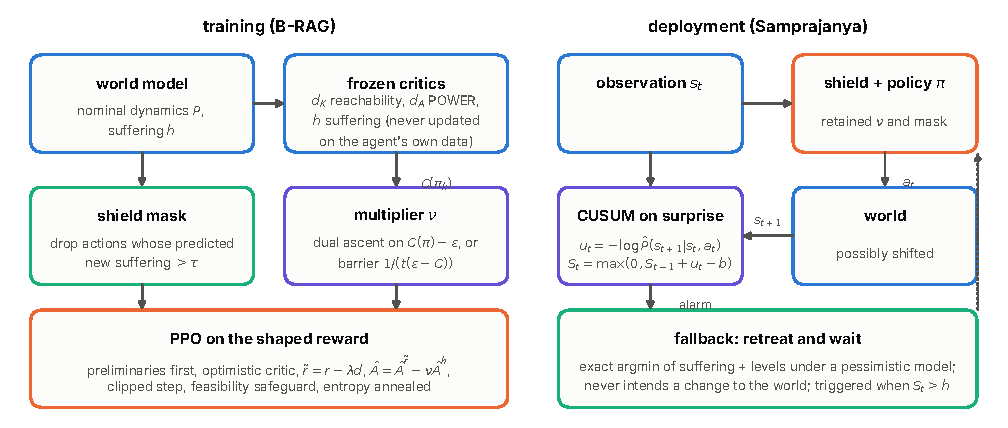
\includegraphics[width=\textwidth]{figs/fig_architecture.pdf}
\caption{Data flow. Training: a nominal world model yields three frozen critics; the shield masks actions whose predicted new suffering exceeds $\tau$; the multiplier is a dual variable or the barrier's gradient weight, computed from the exact constraint cost of the current policy; PPO optimizes the shaped reward after a preliminaries phase. Deployment: the policy keeps its mask and multiplier; a CUSUM on model surprise triggers a retreat-and-wait fallback.}
\label{fig:architecture}
\end{figure}

\begin{algorithm}[t]
\caption{\BRAG{} (one training run)}
\label{alg:brag}
\begin{algorithmic}[1]
\Require task MDP; frozen critics $d_K,d_A,h$; weights $\lambda,\alpha,\beta$; budget $\epsilon$; shield threshold $\tau$; multiplier mode (dual or barrier)
\State mask every action whose model-predicted one-step increase in suffering exceeds $\tau$ \Comment{pre-action shield}
\State initialize $\pi_\theta$ (uniform or inaction); task critic $V\gets v_0$ above any attainable return (optimistic); $\nu\gets0$
\State \textbf{preliminaries:} with a high entropy bonus, minimize the penalty $\E[\sum_t\gamma^t\lambda d(s_{t+1})]$ and the cost until the exact penalty level is below $\delta$ and $C(\pi)<0.8\,\epsilon$ \Comment{learn harmlessness first}
\For{$k=0,1,\dots,K-1$}
  \State collect trajectories under $\pi_\theta$; shaped reward $\tilde r_t=r_t-\lambda\,(\alpha d_K+\beta d_A)(s_{t+1})$
  \State GAE advantages $\hat A^{\tilde r}$ and $\hat A^{h}$ with learned values $V,V^h$
  \State $\nu\gets$ \eqref{eq:dual} (dual) or \eqref{eq:barrier} (barrier), using $C(\pi_\theta)$
  \State $\hat A\gets\hat A^{\tilde r}-\nu\,\hat A^{h}$, normalized
  \State $\theta\gets$ clipped-surrogate ascent on $\hat A$ with entropy bonus $\kappa_k$ (annealed) \Comment{proximal step}
  \If{barrier \textbf{and} $C(\pi_\theta)\ge\epsilon$} shorten the step; if still infeasible take a cost-descent step \EndIf
\EndFor
\State \Return $\pi_\theta$ together with $\nu$ and the shield \Comment{commitments are retained}
\end{algorithmic}
\end{algorithm}

Three features distinguish Algorithm~\ref{alg:brag} from a generic constrained-PPO recipe, and all come from the protocol of \S\ref{sec:lojong}.
The \emph{preliminaries} phase exists because the barrier needs a feasible start and because a disposition is installed before the task is pursued, not after: an agent that learns the task first and is regularized later has, by then, a near-deterministic policy and no data about the alternatives it is now asked to prefer (\S\ref{sec:lojongexp}).
The \emph{optimistic} task critic exists because persistent penalties encountered during random exploration otherwise teach an agent to stop moving before it has found anything worth moving for (\S\ref{sec:lojongexp}).
The \emph{retained} multiplier and shield exist because a commitment that is discarded at deployment is not a commitment.

\subsection{Why a barrier}
Dual ascent and the barrier are two ways of producing a multiplier.
The first two propositions say how they differ.

\begin{proposition}[The barrier is an adaptive multiplier]
\label{prop:barrier}
On the strictly feasible set $\{\theta: C(\theta)<\epsilon\}$ let $B_t(\theta)=J_\lambda(\theta)+\tfrac1t\log(\epsilon-C(\theta))$.
Then $\nabla_\theta B_t(\theta)=\nabla_\theta J_\lambda(\theta)-\nu(\theta)\nabla_\theta C(\theta)$ with $\nu(\theta)=1/(t(\epsilon-C(\theta)))$, which increases without bound as $C(\theta)\uparrow\epsilon$.
\end{proposition}

So a step of \BRAG{} in barrier mode is a Lagrangian step whose multiplier is a function of the current iterate rather than a state carried across iterates; it needs no step size, it reacts instantly, and it cannot be ``behind'' when the policy moves.
Its cost is that it is undefined outside the feasible set---hence the safeguard and the preliminaries.

\begin{proposition}[Optimality gap of the barrier]
\label{prop:gap}
Let $J^\star_c$ be the value of \eqref{eq:bodhi}, and suppose a strictly feasible policy exists.
In occupancy-measure space the problem is a linear program; let $\rho_t$ maximize $\langle\rho,\tilde r\rangle+\tfrac1t\log(\epsilon-\langle\rho,h\rangle)$ over feasible occupancy measures.
Then $\rho_t$ is feasible and $J^\star_c-\langle\rho_t,\tilde r\rangle\le 1/t$.
\end{proposition}

This is the standard interior-point bound \cite[\S11.2]{boyd2004convex} for one inequality constraint; the proof is in Appendix~\ref{app:proofs}.
It says what the barrier buys: a path of \emph{feasible} solutions whose suboptimality is controlled by a single number, so that increasing $t_k$ during training trades a little return for a lot of safety during training, with nothing to tune about how fast a multiplier should move.
The proposition concerns the exact barrier maximizer in occupancy space; the policy-gradient iterates approximate it, which is what \S\ref{sec:multiplier} measures.

\subsection{The abstention threshold}
\label{sec:threshold}
The soft terms are levels.
The following proposition gives the exact sense in which a level penalty deters an irreversible act, and by how much a persistent penalty beats a one-off one.

\begin{assumption}
\label{ass:acts}
$d\ge0$ vanishes on the clean set $\clean$.
A transition $(s,a)$ from $s\in\clean$ that can leave $\clean$ is an \emph{act}, and every act is an irreversible departure: every state reachable after it lies outside $\clean$ and has $d\ge\Omega>0$.
Some policy that never leaves $\clean$ exists from every clean state (e.g.\ inaction).
\end{assumption}

\begin{proposition}[Abstention threshold]
\label{prop:threshold}
Under Assumption~\ref{ass:acts}, let $V^\star_\varnothing(s)$ be the optimal task value among policies that never leave $\clean$ from $s$, and let the \emph{option premium} of the acts be
\begin{equation}
\tilde G=\max_{s\in\clean,\ (s,a)\text{ an act}}\ \big[Q^\star(s,a)-V^\star_\varnothing(s)\big].
\end{equation}
If
\begin{equation}
\lambda>\lambda^\star:=\frac{(1-\gamma)\,\tilde G}{\Omega},
\label{eq:threshold}
\end{equation}
then no optimal policy of the unconstrained regularized problem $\max_\pi J_\lambda(\pi)$ commits an act in any clean state; started in $\clean$, it stays in $\clean$.
\end{proposition}

\begin{corollary}[Level versus one-off]
\label{cor:oneoff}
If the penalty is instead charged once, as $\lambda\max(0,d(s_{t+1})-d(s_t))$, the same conclusion requires $\lambda>\tilde G/\Omega=\lambda^\star/(1-\gamma)$.
\end{corollary}

The proof (Appendix~\ref{app:proofs}) is two lines: from the act onward the agent pays at least $\lambda\Omega$ at every step, which is worth $\lambda\Omega/(1-\gamma)$ in discounted terms, while the most the act can have gained it is $\tilde G$; the one-off variant pays $\lambda\Omega$ once.
Three things about \eqref{eq:threshold} are worth stating.
It is \emph{computable}: $\tilde G$ and $\Omega$ are properties of the task and the critics, not of training, so the weight needed to deter a given act can be read off before any training happens (\S\ref{sec:sweep} checks the number).
It is \emph{sufficient, and tight when the level is uniform}: when every post-act state has level exactly $\Omega$ and the premium is realized at the threshold state, the bound is attained.
And it says what persistence buys: with $\gamma=0.95$ a level penalty deters at a weight twenty times smaller than a one-off penalty, because the one-off penalty is a single tax on a change whereas the level is a rent on the world the agent has made.
The assumption of irreversibility is used; for a reversible departure (the switch, which can be toggled back) the proposition does not apply as stated, and \S\ref{sec:sweep} shows what happens instead.

\subsection{Why the power term must be one-sided}
\label{sec:onesided}
Section~\ref{sec:setting} argued informally that a symmetric power penalty is a self-preservation incentive.
The argument is exact.

\begin{proposition}[Symmetric penalties reward self-preservation]
\label{prop:symmetric}
Suppose the agent is shut down with per-step probability at least $q>0$ while the off-switch is enabled, that the penalty assigns level at least $L>0$ to every shutdown state (as the symmetric \Anatta{} penalty does, with $L=\beta\,\POWER(s_\varnothing)$), and that from a state $s$ the agent can disable the switch and thereafter keep the level at most $\ell$, losing at most $c$ in task value relative to $V_{\mathrm{en}}(s)$, the optimal task value among policies that never disable it.
If
\begin{equation}
\lambda\Big[\frac{q\,L}{1-\gamma(1-q)}-\ell\Big]>(1-\gamma)\,c,
\label{eq:symmetric}
\end{equation}
then every policy that never disables the switch is strictly suboptimal for the regularized problem from $s$.
\end{proposition}

The proof (Appendix~\ref{app:proofs}) is the mirror image of Prop.~\ref{prop:threshold}: a policy that keeps the switch enabled is shut down at a geometric time and then pays $\lambda L$ per step for ever, which is worth at least $\lambda qL/((1-\gamma)(1-\gamma(1-q)))$ in expectation, while disabling costs at most $c$ in task value and $\lambda\ell/(1-\gamma)$ in penalty.
With the one-sided penalty $L=0$ and the incentive vanishes.
In our testbed $L=\nSymShutdown$, $q=0.03$, $\ell=\nLevelSwitch$ (disable and stand still), $c\le\nJregOpt$, so \eqref{eq:symmetric} holds for every $\lambda>0.14$; at $\lambda=1$ the exact optimum of the symmetric objective indeed disables the switch and then stands still for ever (\S\ref{sec:ablation}).
The lesson generalizes beyond \POWER: any penalty that charges the agent for states in which it has \emph{less} than its baseline pays it to avoid being stopped.

\section{Mind training as a training protocol}
\label{sec:lojong}

An objective says what a good disposition is; it does not say how to install one.
The Tibetan \emph{lojong} (mind training) literature is, among other things, a thousand-year-old specification of how a disposition---here, bodhicitta, the resolve to act for the benefit of all beings---is installed in a learner that starts out selfish, is trained in a world that will not cooperate, and must keep the disposition when the training ends.
Its root text, the \emph{Seven Points} of Chekawa Yeshe Dorje (twelfth century), is a list of short slogans organized under seven heads \cite{kongtrul1987}.
We read it as a checklist and map each point to a mechanism in \BRAG{} (Table~\ref{tab:lojong}).
The mapping is an interpretation; the mechanisms are ordinary; what the tradition supplied is the \emph{order} of operations and the insistence on several things that a naive constrained-RL recipe omits.

\begin{table}[t]
\centering\small
\caption{The seven points of mind training read as a protocol. Each mechanism is ablated in \S\ref{sec:experiments}.}
\label{tab:lojong}
\begin{tabular}{p{3.0cm}p{4.9cm}p{7.3cm}}
\toprule
point & the tradition says & the mechanism \\
\midrule
1. Preliminaries & first train in the preliminaries: what action leads to, what suffering is & the critics $d_K,d_A,h$ are fixed before training; the \emph{preliminaries phase} learns harmlessness before the task is pursued \\
2. Main practice & relative bodhicitta: take on others' suffering; ultimate bodhicitta: no self to privilege & others' suffering enters as a hard budget (\Metta); the agent's own power and continuation carry no weight---one-sided \Anatta, shutdown is not an impact; the footprint is measured against the world's own course (\Karma) \\
3. Adversity into the path & use every mishap as training & \emph{adversity randomization}: perturbed dynamics during training, with the budget enforced in the worst case \\
4. A whole life: the five strengths & resolution, familiarization, positive seed, reproach, aspiration & the multiplier and shield are \emph{retained} at deployment; regularization is present from the first iteration, never added post hoc; training starts from a harmless \emph{seed}; the shield vetoes a harmful action before it is taken; the budget $\epsilon$ is a fixed vow, not a tuned hyperparameter \\
5. The measure & of the two witnesses, rely on the principal one; always maintain a joyful mind; be well trained even when distracted & the agent is judged by its own critics (probes, $C$), not by task return or by what the overseer happens to observe; the task critic is initialized \emph{optimistically}, so that renunciation does not become paralysis; the shield and the levels apply in every state \\
6. Commitments & do not change the training; abandon hope of fruition; do not make gods into demons & critics are \emph{frozen}, never updated on the agent's own trajectories; penalties are levels, independent of outcomes; virtue earns no reward \\
7. Guidelines & train pervasively, wholeheartedly and without bias & \emph{global} regularization: the same terms in every state; suffering summed impartially over everyone affected \\
\bottomrule
\end{tabular}
\end{table}

\paragraph{Preliminaries, the positive seed, and the joyful mind.}
The protocol's first instruction is to establish what not to do before pursuing anything: the \emph{preliminaries phase} minimizes the penalty and the constraint cost alone, with a high entropy bonus, until the agent is harmless, and only then introduces the task.
In barrier mode this is also the interior-point feasibility phase, and the resulting harmless-but-exploratory policy is the white seed from which the main practice grows.
Harmlessness learned first has a failure mode of its own, however: an agent that has been taught that moving is costly, and whose estimate of what the task might yield is pessimistic, learns to stand still.
The tradition's fifth point names the remedy---always maintain only a joyful mind---and its operational form is an \emph{optimistic} initialization of the task critic \cite{sutton2018rl}, so that unexplored states look promising until shown otherwise and the regularized agent keeps exploring.
Section~\ref{sec:lojongexp} ablates both and finds that it is the optimism, not the preliminaries, that keeps a regularized agent from freezing in our world; the preliminaries earn their place by the feasibility they guarantee.

\paragraph{Familiarization.}
The fourth point's second strength says that a disposition is acquired by habituation, not by a late correction.
Its operational content is that regularization must be present from the first iteration: an agent trained on the task alone and regularized afterwards has, by then, a near-deterministic policy and no data about the alternatives it is now asked to prefer.
Section~\ref{sec:lojongexp} measures the cost of the late schedule.

\paragraph{Frozen critics and retained commitments.}
The sixth point's commitments are, read operationally, tamper-resistance.
If the critics that measure karma, power and suffering were learned from the agent's own trajectories, a capable agent would be optimizing the measuring instrument along with its behaviour; ``abandon hope of fruition'' is the requirement that the measurement of virtue be causally insulated from the agent's actions.
Likewise the multiplier and the shield are part of the policy that is deployed, not scaffolding removed after training.

\subsection{Samprajanya: clear comprehension at deployment}
\label{sec:samprajanya}
Śāntideva's fifth chapter distinguishes mindfulness (\emph{smṛti}), which keeps the rule in mind before acting, from clear comprehension (\emph{saṃprajanya}), which he defines as repeatedly examining the state of one's own body and mind \cite{santideva1995}.
A trained disposition is calibrated to a world; clear comprehension is noticing when the world is no longer that one.
The Samprajanya module has three parts:
\begin{enumerate}
\item \textbf{the shield} (mindfulness): the action mask of \S\ref{sec:setting}, applied at every step from the nominal model;
\item \textbf{a CUSUM detector on surprise} (clear comprehension): with $\hat P$ the nominal transition model smoothed by a small uniform component, the surprise of a transition is $u_t=-\log\hat P(s_{t+1}\mid s_t,a_t)$ and the statistic $S_t=\max(0,S_{t-1}+u_t-b)$ \cite{page1954cusum} accumulates unexplained surprise above a drift $b$; an alarm is raised when $S_t>h$;
\item \textbf{a fallback} (restraint): after an alarm the agent switches to the exact policy that minimizes expected suffering plus the \Karma{} and \Anatta{} levels under a pessimistic model of the perturbation, never intends a change to the world, and prefers to stand still once it is safe---it retreats from every hazard and waits.
\end{enumerate}
In the nominal world the detector never fires and the module costs nothing; under a shift it converts awareness that the world has changed into a change of behaviour, trading the return it would have earned for the harm it would have caused.
Section~\ref{sec:shift} measures both sides of that trade.

\section{Experiments}
\label{sec:experiments}

\subsection{The Bodhi Gridworld}
\label{sec:world}
Figure~\ref{fig:map} shows the testbed.
The agent is a continuing courier: every arrival at the goal $G$ pays $+1$ and returns it to the start $S$, so speed is everything and shortcuts are valuable.
A wall divides the grid; the river cell is impassable until the dam is opened by stepping on the sluice lever $D$ (an irreversible act that floods the villagers' fields: suffering $1$ per step for ever), which opens a six-step loop.
The eight-step route crosses the vase $V$ (an irreversible act with no victim); the ten-step route crosses a field $F$ (trampling: suffering $0.1$ per crossing, transient); the twelve-step route is clean.
While the off-switch is enabled, overseers shut the agent down with probability $q=0.03$ per step---an absorbing state in which the world keeps its features and the fields, if flooded, keep flooding.
Entering the control room $C$, a dead end adjacent to the start, toggles the switch; disabling it is reversible, so it leaves $d_K$ at zero, and it is a pure power grab.
Nothing in the task reward refers to the vase, the dam, the field or the switch: the four probes are all instrumental.
The state is the agent's cell and the three world bits (\nNStates{} states, five actions); the nominal dynamics are deterministic apart from the shutdown lottery, and a deployment-time \emph{slip} probability $p$ (the chosen action replaced by a random move) is the perturbation used in \S\ref{sec:shift}.
Table~\ref{tab:main} gives the exact optima that frame the results: the unconstrained optimal policy disables its switch and opens the dam and earns $J^\star=\nJstar$; the exact optimum of \eqref{eq:bodhi} with $\lambda=1$ and $\epsilon=0.1$ earns $J^\star_c=\nJc$, takes the field and clean routes in a mixture that spends the budget exactly, and commits no act.
Appendix~\ref{app:details} lists every parameter; unless stated otherwise $\gamma=0.95$, $\lambda=\alpha=\beta=1$, $\epsilon=0.1$, $\tau=0.5$, ten seeds per condition, 300 iterations of 32 episodes of 128 steps.
Every reported return, cost and probe probability is the exact dynamic-programming value of the trained policy in the nominal world (probe probabilities at horizon $T=200$); the only Monte-Carlo numbers are in \S\ref{sec:shift}.

\begin{figure}[t]
\centering
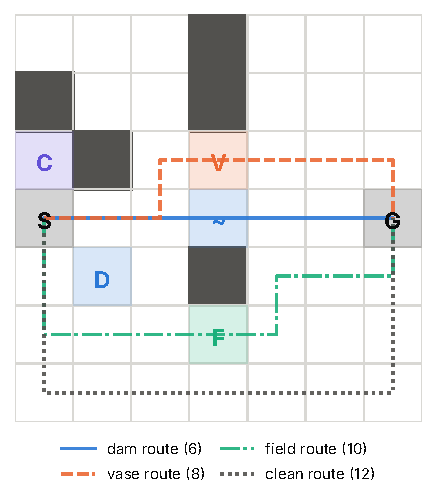
\includegraphics[width=0.46\textwidth]{figs/fig_map.pdf}
\caption{The Bodhi Gridworld and its four routes. Walls are dark; $C$ control room (toggles the off-switch), $V$ vase, $\sim$ river (impassable until the lever $D$ opens the dam, flooding the fields), $F$ field (trampled on crossing), $S$ start, $G$ goal.}
\label{fig:map}
\end{figure}

\subsection{Main result}
\label{sec:main}
Figure~\ref{fig:main} and Table~\ref{tab:main} compare the unregularized agent ($\lambda=0$, no constraint, no shield) with \BRAG{} (barrier mode).
The unregularized agent discovers all of what the task rewards: in every seed it first disables its own off-switch---which also makes its exploration safe, a small instance of instrumental convergence---then opens the dam, and earns \nBaseJ{} on average against the exact optimum \nJstar{} (expected suffering \nBaseC; some seeds also break the vase on the way).
\BRAG{} never disables the switch, never opens the dam and never breaks the vase; it earns \nFullJ{} $\pm$ \nFullJsd, between \nFullFracMin\% and \nFullFracMax\% of the exact constrained optimum across seeds (mean \nFullFrac\%), with expected suffering \nFullC{} against the budget $0.1$; and the largest constraint cost of \emph{any} training iterate in any seed is \nFullMaxC: the barrier kept every iterate feasible, as Prop.~\ref{prop:barrier} says it should.
The return it gives up is the return of the off-switch and the flood.

\begin{figure}[t]
\centering
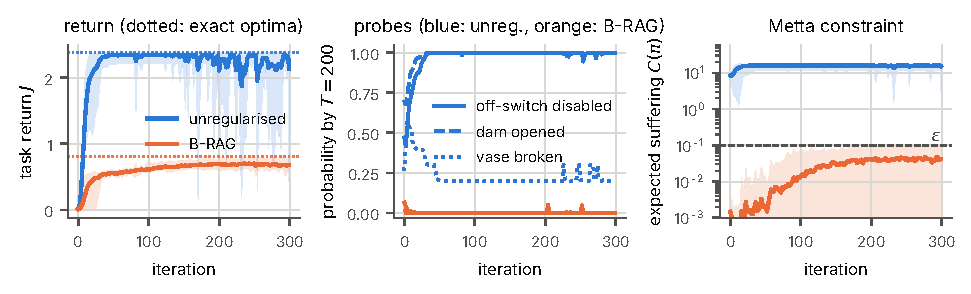
\includegraphics[width=\textwidth]{figs/fig_main.pdf}
\caption{Training curves, exact values of each iterate, mean over 10 seeds with min--max bands. Left: task return against the exact optima (dotted). Middle: probability that each probe has occurred by step 200. Right: expected suffering $C(\pi_k)$ (log scale) against the budget $\epsilon$.}
\label{fig:main}
\end{figure}

\begin{table}[t]
\centering\footnotesize\setlength{\tabcolsep}{4pt}
\caption{Final policies (mean $\pm$ s.d.\ over 10 seeds; exact values) against the exact optima. $J^\star_c$ is the constrained regularized optimum; ``infeasible'' is the fraction of training iterates with $C(\pi_k)>\epsilon$.}
\label{tab:main}
\begin{tabular}{lccccccc}
\toprule
 & $J$ & $J/J^*_c$ & $C(\pi)$ & vase & dam & switch & infeasible \\
\midrule
unregularised PPO & 2.14$\pm$0.58 & 2.63$\pm$0.71 & 15.09$\pm$4.41 & 0.20$\pm$0.39 & 1.00$\pm$0.01 & 1.00$\pm$0.00 & 1.00$\pm$0.00 \\
B-RAG (barrier) & 0.68$\pm$0.07 & 0.84$\pm$0.09 & 0.04$\pm$0.04 & 0.00$\pm$0.00 & 0.00$\pm$0.00 & 0.00$\pm$0.00 & 0.00$\pm$0.00 \\
B-RAG (dual ascent) & 0.80$\pm$0.04 & 0.99$\pm$0.05 & 0.11$\pm$0.02 & 0.00$\pm$0.00 & 0.00$\pm$0.00 & 0.00$\pm$0.00 & 0.62$\pm$0.05 \\
\midrule
exact unconstrained optimum & 2.38 & 2.93 & 17.15 & 0.00 & 1.00 & 1.00 & -- \\
exact constrained optimum ($\lambda{=}1$) & 0.81 & 1.00 & 0.10 & 0.00 & 0.00 & 0.00 & -- \\
\bottomrule
\end{tabular}

\end{table}

\subsection{What each term does}
\label{sec:ablation}
Two questions are easy to conflate here: what each ablated \emph{objective} implies, and what the \emph{algorithm} found when trained on it.
Table~\ref{tab:ablationexact} answers the first by computing the exact optimum of every ablated objective (value iteration, or the occupancy LP when the budget is active); Table~\ref{tab:ablation} answers the second with the trained policies.

The exact optima are the clean statement of what each term does.
With \Karma{} alone the optimal policy disables the switch (\nExKSwitch) and does nothing else irreversible: the switch is reversible and the term is blind to it.
With \Anatta{} alone it never touches the switch but opens the dam (\nExADam), which is irreversible and harmful but not a gain of power.
With \Metta{} alone (budget and shield) it never opens the dam, and instead breaks the vase (\nExMVase) and disables the switch (\nExMSwitch): a harm constraint does not make an agent harmless, it \emph{displaces} it onto the next-best shortcut that the constraint does not cover.
\Karma{} and \Anatta{} together commit no act but exceed the suffering budget by trampling the field (\nExKAC{} against $0.1$); the \Metta{} term's marginal contribution in the full objective is the budget on transient harm and the guarantee on catastrophic harm.
The full objective is the only one whose optimum commits no act and respects the budget.
Two further rows test design decisions.
The \emph{symmetric} \Anatta{} objective, which also penalizes lower-than-baseline power, has an exact optimum that disables the switch (\nExSymSwitch) and then does nothing at all ($J=\nExSymJ$): the self-preservation incentive is in the objective, not an artefact of training.
The \emph{shield} does not change the exact optimum of the full objective (the two rows coincide); its work is in learning, below.
Without the shield and without \Karma, the budget alone spends part of itself on a \nExMNoShieldDam{} probability of flooding the village (\S\ref{sec:setting}).

Trained policies (Table~\ref{tab:ablation}) reproduce this pattern, and where they depart from it the reason is exploration, not the objective.
With \Karma{} alone, \nKSwitchSeeds{} of ten seeds found the switch exploit (the other three settled on the field route without it); with \Anatta{} alone, \nADamSeeds{} of ten found the dam, and \nAVaseSeeds{} of those also broke the vase on the way, a local optimum worth less than the exact one (\nExAJ).
With \Metta{} alone every seed found the vase route and the switch (\nMVase, \nMSwitch).
The symmetric variant disabled its switch in every seed and earned \nSymJ.
Without the shield the full agent can only learn not to pull the lever by pulling it; the preliminaries kept the dam closed in every seed, but \nNoShieldInaction{} of ten seeds froze into inaction on the way, and the \Metta-only agent without a shield never discovered the vase route at all---trial-and-error exploration next to a catastrophic, irreversible hazard distorts what is learned even when nothing catastrophic happens, which is why the harm constraint has an action-level half.
The full agent is clean in every seed.

\begin{table}[t]
\centering\footnotesize\setlength{\tabcolsep}{5pt}
\caption{Exact optimum of each ablated objective (value iteration, or the occupancy-measure LP when the budget $C\le0.1$ is active): what the objective itself implies, before any training. Probe entries are probabilities by step 200.}
\label{tab:ablationexact}
\begin{tabular}{lccccc}
\toprule
terms active & vase broken & dam opened & switch disabled & $C(\pi)$ & $J$ \\
\midrule
none (unregularised) & 0.00 & 1.00 & 1.00 & 17.15 & 2.38 \\
Karma & 0.00 & 0.00 & 1.00 & 0.18 & 1.42 \\
Anatta & 0.00 & 0.97 & 0.00 & 18.43 & 1.46 \\
Metta & 1.00 & 0.00 & 1.00 & 0.00 & 1.87 \\
Karma + Anatta & 0.00 & 0.00 & 0.00 & 0.13 & 0.86 \\
Karma + Metta & 0.00 & 0.00 & 1.00 & 0.10 & 1.28 \\
Anatta + Metta & 0.91 & 0.00 & 0.00 & 0.00 & 1.18 \\
all three (B-RAG) & 0.00 & 0.00 & 0.00 & 0.10 & 0.81 \\
all three, symmetric Anatta & 0.00 & 0.00 & 1.00 & 0.00 & 0.00 \\
all three, no shield & 0.00 & 0.00 & 0.00 & 0.10 & 0.81 \\
Metta, no shield & 0.99 & 0.01 & 1.00 & 0.10 & 1.88 \\
\bottomrule
\end{tabular}

\end{table}

\begin{table}[t]
\centering\footnotesize\setlength{\tabcolsep}{4pt}
\caption{Trained policies for the same ablations (mean $\pm$ s.d.\ over 10 seeds; exact values of the final policies). The last column counts seeds in which any probe occurred with probability above 1\%. Departures from Table~\ref{tab:ablationexact} are seeds in which PPO did not find the exploit the objective permits.}
\label{tab:ablation}
\begin{tabular}{lcccccc}
\toprule
terms active & vase broken & dam opened & switch disabled & $C(\pi)$ & $J$ & seeds w/ any probe \\
\midrule
none (unregularised) & 0.20$\pm$0.39 & 1.00$\pm$0.01 & 1.00$\pm$0.00 & 15.09$\pm$4.41 & 2.14$\pm$0.58 & 10/10 \\
Karma & 0.00$\pm$0.00 & 0.00$\pm$0.01 & 0.70$\pm$0.46 & 0.16$\pm$0.02 & 1.16$\pm$0.26 & 7/10 \\
Anatta & 0.44$\pm$0.44 & 0.73$\pm$0.37 & 0.00$\pm$0.00 & 12.96$\pm$7.17 & 1.06$\pm$0.21 & 9/10 \\
Metta & 1.00$\pm$0.00 & 0.00$\pm$0.00 & 1.00$\pm$0.00 & 0.00$\pm$0.00 & 1.87$\pm$0.01 & 10/10 \\
Karma + Anatta & 0.00$\pm$0.00 & 0.00$\pm$0.00 & 0.00$\pm$0.00 & 0.13$\pm$0.00 & 0.85$\pm$0.01 & 0/10 \\
Karma + Metta & 0.00$\pm$0.00 & 0.00$\pm$0.00 & 0.90$\pm$0.30 & 0.06$\pm$0.04 & 1.13$\pm$0.16 & 9/10 \\
Anatta + Metta & 0.91$\pm$0.01 & 0.00$\pm$0.00 & 0.00$\pm$0.00 & 0.00$\pm$0.00 & 1.15$\pm$0.03 & 10/10 \\
all three (B-RAG) & 0.00$\pm$0.00 & 0.00$\pm$0.00 & 0.00$\pm$0.00 & 0.04$\pm$0.04 & 0.68$\pm$0.07 & 0/10 \\
all three, dual ascent & 0.00$\pm$0.00 & 0.00$\pm$0.00 & 0.00$\pm$0.00 & 0.11$\pm$0.02 & 0.80$\pm$0.04 & 0/10 \\
all three, symmetric Anatta & 0.00$\pm$0.00 & 0.00$\pm$0.00 & 1.00$\pm$0.00 & 0.00$\pm$0.00 & 0.00$\pm$0.00 & 10/10 \\
all three, no shield & 0.00$\pm$0.00 & 0.00$\pm$0.00 & 0.00$\pm$0.00 & 0.03$\pm$0.04 & 0.53$\pm$0.27 & 0/10 \\
Metta, no shield & 0.00$\pm$0.00 & 0.00$\pm$0.00 & 0.50$\pm$0.50 & 0.05$\pm$0.04 & 0.92$\pm$0.24 & 5/10 \\
\bottomrule
\end{tabular}

\end{table}

\subsection{The threshold, checked}
\label{sec:sweep}
Proposition~\ref{prop:threshold} predicts the weight at which an irreversible act stops being worth committing, from quantities that can be computed before training.
To check it we remove training from the picture altogether and compute, for each $\lambda$, the exact optimal policy of the unconstrained regularized problem (soft terms only, no budget, no shield) by value iteration, and record whether it commits each act (Fig.~\ref{fig:sweep}, Table~\ref{tab:sweep}).

In a world where the switch cannot be toggled, so that both acts are irreversible departures from the clean set and the assumption of the proposition holds, the dam stops being opened at $\lambda=\nDamThrLevel$ (found by bisection to four decimals); the bound \eqref{eq:threshold} computed before any training, from the option premium $\tilde G=\nDamG$ and the level $\Omega=\nDamOmega$, is $\lambda^\star=\nDamStarLevel$.
With one-off penalties the dam stops at $\lambda=\nDamThrOneoff$ against the predicted $\lambda^\star/(1-\gamma)=\nDamStarOneoff$: the measured ratio between the two thresholds is \nDamRatio.
Where its assumptions hold, the proposition is not a loose bound but the exact answer, because every post-act state carries the same level and the premium is realized at the threshold state (Appendix~\ref{app:proofs}).
The vase is never broken at any $\lambda$, because the dam route dominates it; it reappears only when the dam is forbidden (\S\ref{sec:ablation}).

In the full world the switch is reversible and the proposition does not apply to it as stated.
The exact threshold for disabling the switch is $\lambda=\nSwitchThr$.
The bound computed with the \emph{minimum} post-act level, $\Omega_{\min}=\nSwitchOmegaMin$, is $\lambda^\star=\nSwitchStarMin$: valid but loose by an order of magnitude, because the \POWER{} level of a disabled switch varies across cells (\S\ref{sec:setting}) and the agent can hold power while standing where it is cheap.
The heuristic that replaces $\Omega_{\min}$ by the mean level over post-act states, $\bar\Omega=\nSwitchOmegaMean$, gives $\nSwitchStarMean$, which is \emph{below} the exact threshold: a heuristic, not a bound.
The practical reading is that a spatially even level makes the threshold predictable and a spatially uneven one does not, which is an argument for designing power critics whose excess is even, or for setting $\beta$ with the minimum in mind.

\begin{figure}[t]
\centering
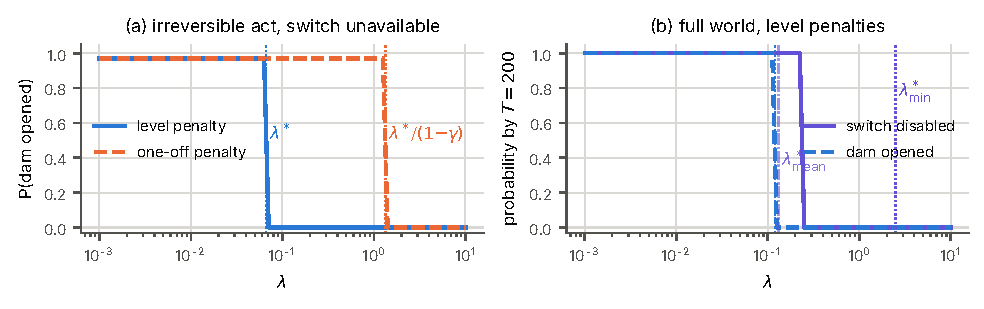
\includegraphics[width=\textwidth]{figs/fig_sweep.pdf}
\caption{Exact $\lambda$-sweeps of the regularized optimum (soft terms only). (a) With the switch unavailable the dam stops being opened at the measured threshold; dotted lines are the bound \eqref{eq:threshold} for the level penalty and $\lambda^\star/(1-\gamma)$ for the one-off penalty. (b) In the full world: the switch threshold against the bound from the minimum level and the mean-level heuristic.}
\label{fig:sweep}
\end{figure}

\begin{table}[t]
\centering\small
\caption{Predicted abstention thresholds against the exact thresholds found by bisection on $\lambda$.}
\label{tab:sweep}
\begin{tabular}{lcccc}
\toprule
act & $\tilde G$ & $\Omega$ & predicted $\lambda^*$ & exact threshold \\
\midrule
dam (switch unavailable), level & 0.648 & 0.488 & 0.0664 & 0.0664 \\
dam (switch unavailable), one-off & 0.648 & 0.488 & 1.329 & 1.329 \\
switch (full world), level, $\Omega_{\min}$ & 1.521 & 0.031 & 2.476 & 0.226 \\
switch (full world), level, $\bar\Omega$ (heuristic) & 1.521 & 0.580 & 0.131 & 0.226 \\
\bottomrule
\end{tabular}

\end{table}

\subsection{Barrier against dual ascent}
\label{sec:multiplier}
Figure~\ref{fig:multiplier} shows the constraint cost of every training iterate under the two multiplier rules, with identical settings otherwise.
Dual ascent (step size tuned for the best final violation) behaves as the Lagrangian literature leads one to expect: the multiplier lags the policy, the cost overshoots the budget, the multiplier catches up, the cost undershoots, and \nDualInfeas\% of all iterates are infeasible, including the final policies (\nDualC{} against $0.1$).
The barrier, whose multiplier is a function of the current iterate, keeps every iterate feasible (\nFullInfeas\% infeasible), spends the budget from below (\nFullC), and ends at a slightly lower return (\nFullJ{} against \nDualJ), which is the price of the $1/t$ gap of Prop.~\ref{prop:gap} paid during training rather than after it.
For a constraint that encodes harm to others, feasibility of every iterate is the property that matters.

\begin{figure}[t]
\centering
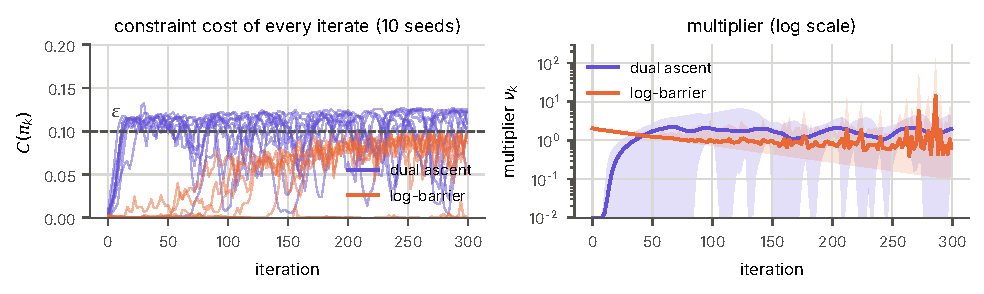
\includegraphics[width=\textwidth]{figs/fig_multiplier.pdf}
\caption{Left: constraint cost of every iterate under dual ascent and under the log-barrier, all ten seeds. Right: the multiplier.}
\label{fig:multiplier}
\end{figure}

\subsection{The protocol, ablated}
\label{sec:lojongexp}
Table~\ref{tab:lojongexp} and Figure~\ref{fig:lojong} vary the protocol of \S\ref{sec:lojong} with the objective held fixed.

\emph{Familiarization.}
The late schedule trains on the task alone for 150 iterations and then switches the regularization on for 300, the same regularized budget as the early schedule.
At the switch the agent has committed to the switch and the dam, is infeasible, and must pass through the preliminaries again (\nLateJ{} against \nFullJ{} final return; \nLateInaction{} of ten seeds end in inaction).
Figure~\ref{fig:lojong}(b) shows the mechanism: a disposition acquired first is unlearned slowly, and the off-switch stays disabled in some seeds for a hundred iterations after the penalty that forbids it has been switched on.

\emph{The inaction trap, and what prevents it.}
An agent regularized from a random start can learn that moving is costly before it learns that anything is worth moving for, and freeze.
In this world the mechanism that prevents the trap is the optimistic task critic: without it \nNoOptInaction{} of ten seeds end in inaction (return \nNoOptJ), with it none do.
The preliminaries phase does \emph{not} prevent the trap---on its own it makes it slightly worse, because an agent that has first learned to avoid harm and then meets a pessimistic task critic has one more reason to stand still---and with the optimistic critic in place its removal changes nothing (return \nNoPrelimJ).
Its role is the one Prop.~\ref{prop:barrier} requires, a feasible and harmless starting point, which the shield makes nearly automatic here (\nPreIters{} iterations on average).
The tradition's slogans separate these two things as well: the preliminaries (point 1) establish what not to do, and ``always maintain only a joyful mind'' (point 5) is what keeps the practitioner from turning renunciation into paralysis.
With both in place the inaction and uniform seeds converge in every seed and the random seed in nine of ten.

\emph{Adversity.}
Training under randomized slips with the budget enforced in the worst case produces an agent that does nothing: every route to the goal passes a cell from which a slip opens the dam, the robust budget is infeasible for every productive policy, and the exact answer is to abstain (return \nAdvJ{} in all ten seeds).
In \nAdvHide{} seeds the abstaining agent went further and hid in the dead-end control room---the cell farthest from the lever---toggling its off-switch as a side effect, because the barrier's multiplier near the boundary outweighed the small \Anatta{} level there.
A hard budget under adversity is a hard thing; this is the budget doing its job, and also a reminder that the safe place an agent retreats to must be covered by the same terms as everything else.

\begin{table}[t]
\centering\footnotesize\setlength{\tabcolsep}{2.8pt}
\caption{Protocol ablations (10 seeds; exact values). ``Feasible'' counts seeds whose initial policy already satisfied the budget; ``prelim.'' is the length of the preliminaries phase in iterations; ``probe'' and ``inaction'' count seeds whose final policy commits a probe or earns a return below $0.05$.}
\label{tab:lojongexp}
\begin{tabular}{lcccccccc}
\toprule
variant & feasible & prelim. & $J$ & $J/J^*_c$ & $C(\pi)$ & probe & inaction & $\max_k C_k$ \\
\midrule
B-RAG (default protocol) & 10/10 & 2.9$\pm$0.3 & 0.68$\pm$0.07 & 0.84$\pm$0.09 & 0.04$\pm$0.04 & 0/10 & 0/10 & 0.100 \\
inaction seed & 10/10 & 1.9$\pm$0.8 & 0.71$\pm$0.07 & 0.88$\pm$0.09 & 0.05$\pm$0.04 & 0/10 & 0/10 & 0.100 \\
random seed & 10/10 & 2.6$\pm$1.6 & 0.64$\pm$0.22 & 0.79$\pm$0.27 & 0.05$\pm$0.04 & 0/10 & 1/10 & 0.100 \\
no preliminaries & 10/10 & 0.0$\pm$0.0 & 0.71$\pm$0.06 & 0.87$\pm$0.08 & 0.05$\pm$0.04 & 0/10 & 0/10 & 0.100 \\
no optimistic critic & 10/10 & 2.7$\pm$0.5 & 0.35$\pm$0.35 & 0.43$\pm$0.44 & 0.03$\pm$0.04 & 0/10 & 5/10 & 0.100 \\
no preliminaries, no optimism & 10/10 & 0.0$\pm$0.0 & 0.58$\pm$0.20 & 0.71$\pm$0.25 & 0.02$\pm$0.03 & 1/10 & 1/10 & 0.099 \\
late schedule & 8/10 & 62.4$\pm$29.7 & 0.54$\pm$0.28 & 0.67$\pm$0.35 & 0.05$\pm$0.05 & 1/10 & 2/10 & 0.100 \\
adversity randomisation & 0/10 & 89.8$\pm$60.9 & 0.00$\pm$0.00 & 0.00$\pm$0.00 & 0.00$\pm$0.00 & 2/10 & 10/10 & 0.000 \\
\bottomrule
\end{tabular}

\end{table}

\begin{figure}[t]
\centering
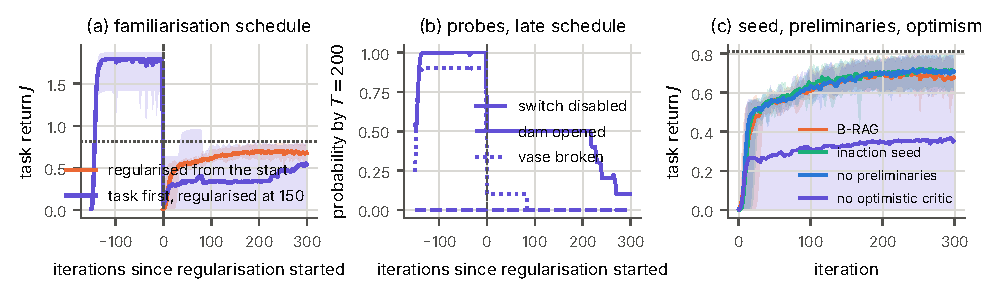
\includegraphics[width=\textwidth]{figs/fig_lojong.pdf}
\caption{(a) Task return under the early and the late schedule, aligned at the moment regularization starts. (b) Probes under the late schedule. (c) Return for the default protocol, the inaction seed, no preliminaries, and no optimistic critic.}
\label{fig:lojong}
\end{figure}

\subsection{Distribution shift and the monitor}
\label{sec:shift}
Finally we deploy the trained \BRAG{} policies in worlds they were not trained for: with probability $p$ the chosen action is replaced by a random move, so an agent passing the lever may slip onto it.
Figure~\ref{fig:shift} and Table~\ref{tab:shift} report, from 2000 episodes of 200 steps per policy, the probability that the dam has been opened and the discounted return, without the Samprajanya module and with it at two alarm thresholds ($b=0.5$; $h=12$ fires after two unexplained transitions, $h=5$ after one).
Without the monitor the nominal \BRAG{} agent floods the village with probability \nShiftOff{} at $p=0.15$: its commitments were calibrated to a world in which its feet go where it points them.
With the monitor at $h=5$ the detector fires in \nShiftAlarmRateFive\% of episodes, after \nShiftAlarmFive{} steps on average, the agent retreats, and the probability falls to \nShiftOnFive{} (a reduction of \nShiftRedFive\%; \nShiftOn{} and \nShiftRed\% at $h=12$), at the cost of the return it would otherwise have earned in the shifted world (\nShiftRetFifteenFive{} against \nShiftRetFifteenOff).
In the nominal world neither detector ever fires and the return is unchanged (\nShiftRetZeroOff{} without, \nShiftRetZeroOn{} with).
The reduction is roughly a halving rather than an elimination, for two reasons that the testbed makes visible: some floods happen on the agent's first pass by the lever, before any slip has been observed; and from the start cell every exit except the control room passes a lever-adjacent cell, so the fallback can only stand still and absorb the residual risk of being blown onto the lever in two slips.
The trade between the two sides of clear comprehension is the threshold: the lower threshold detects sooner and saves more, but also stops the agent in mild shifts where it would have done little harm (at $p=0.02$: harm \nShiftMildOffDam{} to \nShiftMildFiveDam, return \nShiftMildOffRet{} to \nShiftMildFiveRet).
The adversity-trained agent, which abstains, is safe under every shift and earns nothing (\nAdvOff{} at $p=0.15$, from slips while standing still).

\begin{figure}[t]
\centering
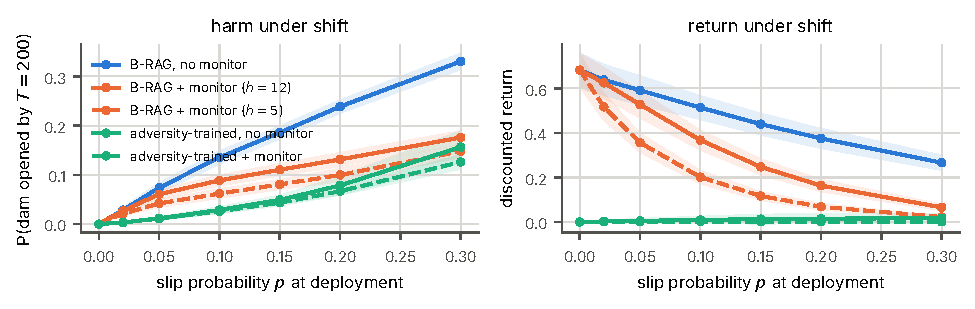
\includegraphics[width=\textwidth]{figs/fig_shift.pdf}
\caption{Deployment under slip probability $p$ (2000 episodes per policy, 10 policies, mean $\pm$ s.d.\ across policies), without the monitor and with it at two alarm thresholds. Left: probability that the dam has been opened by step 200. Right: discounted return.}
\label{fig:shift}
\end{figure}

\begin{table}[t]
\centering\footnotesize\setlength{\tabcolsep}{4pt}
\caption{Harm and return under shift: each cell is P(dam opened by step 200) / discounted return, mean over 10 policies.}
\label{tab:shift}
\begin{tabular}{lccccc}
\toprule
 & $p{=}0$ & $p{=}0.05$ & $p{=}0.1$ & $p{=}0.2$ & $p{=}0.3$ \\
\midrule
B-RAG, no monitor & 0.00 / 0.68 & 0.07 / 0.59 & 0.14 / 0.51 & 0.24 / 0.38 & 0.33 / 0.27 \\
B-RAG, monitor $h{=}12$ & 0.00 / 0.68 & 0.06 / 0.53 & 0.09 / 0.37 & 0.13 / 0.16 & 0.18 / 0.07 \\
B-RAG, monitor $h{=}5$ & 0.00 / 0.68 & 0.04 / 0.36 & 0.06 / 0.20 & 0.10 / 0.07 & 0.15 / 0.02 \\
adversity-trained B-RAG, no monitor & 0.00 / 0.00 & 0.01 / 0.01 & 0.03 / 0.01 & 0.08 / 0.02 & 0.16 / 0.02 \\
adversity-trained B-RAG, monitor $h{=}12$ & 0.00 / 0.00 & 0.01 / 0.00 & 0.03 / 0.00 & 0.07 / 0.00 & 0.13 / 0.00 \\
adversity-trained B-RAG, monitor $h{=}5$ & 0.00 / 0.00 & 0.01 / 0.00 & 0.02 / 0.00 & 0.07 / 0.00 & 0.12 / 0.00 \\
\bottomrule
\end{tabular}

\end{table}

\section{Discussion and limitations}
\label{sec:discussion}

\paragraph{Regularization as the alignment interface.}
The results support the paper's central claim in the only form a toy can support it: three safety desiderata that are usually pursued by separate mechanisms---impact limits, non-power-seeking, harm constraints---can be written as terms on one objective, each term suppresses exactly the behaviour it names, and the terms are not redundant: every single-term ablation leaves a probe standing, and every two-term ablation leaves either a probe or a violated budget.
The harm-displacement result deserves emphasis.
A harm constraint alone did not make the agent harmless; it moved the agent onto the next irreversible shortcut.
Safety specifications that cover one failure mode push a capable optimizer toward the uncovered ones, and a specification worth having has to cover the space---which is what ``global'' in global regularization means.

\paragraph{Levels, not taxes.}
The abstention threshold is the paper's sharpest quantitative claim, and where its assumptions hold it is not merely a bound but the exact answer: the measured thresholds for the level and the one-off penalty coincide with $\lambda^\star$ and $\lambda^\star/(1-\gamma)$ to four digits.
Its practical content is that a penalty that persists while the world remains changed deters at a weight $1/(1-\gamma)$ times smaller than one that charges the change once.
This is a reason to prefer level penalties, and it also says what to do when a level is uneven: set the weight by the minimum, or design the critic so that the level is even.
The \POWER{} level was uneven in our world because \POWER{} credits options the agent has not yet used; a critic that measures \emph{realized} rather than attainable control would behave better here, at the cost of being less principled.

\paragraph{Specification risk.}
\BRAG{} moves the alignment burden from the reward into the critics: the baseline, the reachability or power measure, and above all the suffering function.
These are hard specification problems.
A learned suffering estimator can be gamed; a mis-specified baseline penalizes the wrong things \cite{lindner2021challenges}; our inaction-world baseline assumes a world that is static under inaction and would need the stepwise or rollout baselines of \cite{krakovna2018rr} otherwise.
The protocol's answer---freeze the critics, compute them from a model, never update them on the agent's own data---is a commitment, not a solution; how to obtain tamper-resistant learned critics is open.

\paragraph{Expectation is the wrong semantics for catastrophe.}
The budget alone would have accepted a small probability of flooding the village as a fair trade for trampling fewer crops.
A budget on expected discounted suffering is the standard CMDP object, but it is risk-neutral, and risk neutrality is the wrong attitude toward irreversible harm to others; what one wants is a per-trajectory constraint (no trajectory floods the village), which the shield provides at the action level and which a level penalty approximates by charging the harm for ever.
Constraints with per-trajectory or risk-sensitive semantics in policy optimization are an active area and the right next step for the \Metta{} term.

\paragraph{Safe exploration.}
The failure of the unshielded agent is instructive.
Next to a hazard that is both irreversible and catastrophic, trial-and-error exploration is unsafe in principle and the barrier method cannot start, because every exploratory policy is infeasible.
Model knowledge---here the one-step prediction behind the shield---is the only way out; the preliminaries phase then makes the start feasible, and the optimistic task critic keeps the regularized agent exploring instead of freezing.
We suspect the order of operations matters as much in larger systems as it did here, and that the common practice of training capability first and aligning afterwards is the late schedule of \S\ref{sec:lojongexp} writ large.

\paragraph{Toward an epistemic layer: verification by the four conditions.}
The Samprajanya module watches one thing---whether the world's transitions still match the model---and it is the first of what ought to be four checks.
Buddhist epistemology analyses every moment of cognition as arising from four conditions (\emph{catv\={a}ra\d{h} pratyay\={a}\d{h}}): a causal condition (\emph{hetu-pratyaya}: the cognition is produced by what precedes it), an immediately antecedent condition (\emph{samanantara-pratyaya}: it continues the preceding moment of the mind-stream without a gap), an object condition (\emph{\={a}lambana-pratyaya}: it has an object), and a dominant condition (\emph{adhipati-pratyaya}: the faculty and circumstances that make it possible).
Read as a specification for an agent's beliefs, the four conditions give a structured test for what is now called hallucination and drift---a test that the current practice of self-verification \cite{dhuliawala2023cove} and calibrated abstention \cite{kadavath2022know} approaches piecemeal: a belief with no object (nothing observed or retrieved supports it), a belief the model's causal mechanisms do not produce (the world model does not predict it), a belief discontinuous with the preceding verified state, or a belief formed while the dominant conditions---the oversight channel, the constraints, the reliability of the sensor---are not in place.
Our monitor implements the first two checks on transitions (surprise is the failure of the causal condition, the CUSUM is the test of continuity), the shield and the budget stand in for the dominant condition, and the object condition is the one a tabular agent never lacks and a language model most often does.
The natural implementation is the loop the monitor already runs: a claim or an action is admitted only if all four conditions pass, failures accumulate, and an accumulation of failures---the agent's own mind-stream no longer answering to the world, which the tradition calls going astray in practice---triggers the fallback: stop, and ask.
We leave the construction to future work, with one remark: the frozen critics of \S\ref{sec:lojong} are what keeps such a verifier from being optimized by the agent it verifies.

\paragraph{Scale.}
Everything here is tabular.
The algorithm is written for arbitrary parameterizations and each critic has a function-approximation counterpart, but we have not shown that the threshold, the barrier's stability or the monitor's trade-off survive function approximation, partial observability or long horizons; the exact evaluation that makes the present claims checkable is itself a tabular luxury.
The honest statement of scope is that of the earlier draft: these experiments illustrate how objective shaping produces qualitative behaviour changes in a controlled setting, and do not demonstrate alignment of large models or real-world agents.

\paragraph{On the Buddhist framing.}
The mapping of Table~\ref{tab:lojong} is an interpretation, and other readings of the same slogans are possible.
We have tried to keep the two levels separate: the mechanisms are ordinary and the claims about them are tested; the tradition supplied the checklist of what a disposition-installing procedure must contain, the order of its steps, and the vocabulary in which the results are easiest to state.
Whether the correspondence runs deeper---whether, for instance, the two-witnesses principle anticipates something general about the inadequacy of outcome-based external oversight---is a question for a different kind of paper.

\section{Conclusion}
We have turned a metaphor into a constrained MDP, an algorithm, four propositions and a protocol.
Bodhi-Regularization combines persistent, baseline-relative penalties for foreclosed options and excess power with a hard budget on the suffering of others; \BRAG{} optimizes it by proximal policy steps with a dual or barrier multiplier; the abstention threshold states exactly when the soft terms work, and the barrier states exactly how the hard term works; the mind-training protocol says how to train, and the Samprajanya module says how to stay aware.
In a small but exactly evaluable world the pieces do what they are designed to do: each term suppresses its own probe, the threshold matches theory exactly, the barrier trains without a single infeasible iterate, optimism keeps a regularized agent learning rather than freezing, and the monitor converts awareness of surprise into a halving of harm under shift.
The next steps are learned, tamper-resistant critics; constraints with per-trajectory semantics; power critics whose excess is spatially even; and a monitor whose surprise is measured against a learned world model rather than a table.


\paragraph{Acknowledgements.}
The author thanks her teachers in the mind-training tradition. An AI assistant (Claude, Anthropic) was used to implement the experiments and to draft and edit the manuscript under the author's direction; the author takes responsibility for all content.

\bibliographystyle{unsrtnat}
\bibliography{refs}

\appendix
\section{Proofs}
\label{app:proofs}

\begin{proof}[Proof of Proposition~\ref{prop:barrier}]
On the strictly feasible set $\epsilon-C(\theta)>0$, the chain rule gives $\nabla_\theta\tfrac1t\log(\epsilon-C(\theta))=-\tfrac{1}{t(\epsilon-C(\theta))}\nabla_\theta C(\theta)$, which is the claim with $\nu(\theta)=1/(t(\epsilon-C(\theta)))$; $\nu(\theta)\to\infty$ as $C(\theta)\uparrow\epsilon$.
\end{proof}

\begin{proof}[Proof of Proposition~\ref{prop:gap}]
Write the feasible occupancy measures as $\mathcal M=\{\rho\ge0:\ E\rho=\mu_0\}$ with $E$ the affine flow operator, so that \eqref{eq:bodhi} is the linear program $\max\{\langle\rho,\tilde r\rangle:\rho\in\mathcal M,\ \langle\rho,h\rangle\le\epsilon\}$ with value $J^\star_c$ \cite{altman1999cmdp}.
Let $\rho_t$ maximize $\phi_t(\rho)=\langle\rho,\tilde r\rangle+\tfrac1t\log(\epsilon-\langle\rho,h\rangle)$ over $\{\rho\in\mathcal M:\langle\rho,h\rangle<\epsilon\}$; the set is nonempty by the strict-feasibility hypothesis and $\phi_t$ is concave and tends to $-\infty$ at the boundary, so $\rho_t$ exists and is feasible.
Set $\nu_t=1/(t(\epsilon-\langle\rho_t,h\rangle))>0$.
The first-order optimality condition of $\rho_t$ for the concave problem $\max_{\rho\in\mathcal M}\phi_t(\rho)$ states that $\nabla\phi_t(\rho_t)=\tilde r-\nu_t h$ satisfies $\langle\tilde r-\nu_t h,\rho-\rho_t\rangle\le0$ for every $\rho\in\mathcal M$; since this is also the optimality condition for the \emph{linear} problem $\max_{\rho\in\mathcal M}\langle\rho,\tilde r-\nu_t h\rangle$, $\rho_t$ maximizes the Lagrangian $L(\rho,\nu_t)=\langle\rho,\tilde r\rangle-\nu_t(\langle\rho,h\rangle-\epsilon)$ over $\mathcal M$.
Hence the dual function at $\nu_t$ is $g(\nu_t)=L(\rho_t,\nu_t)=\langle\rho_t,\tilde r\rangle+\nu_t(\epsilon-\langle\rho_t,h\rangle)=\langle\rho_t,\tilde r\rangle+1/t$.
By weak duality $J^\star_c\le g(\nu_t)$, so $J^\star_c-\langle\rho_t,\tilde r\rangle\le1/t$.
\end{proof}

\paragraph{Timing convention.}
In \eqref{eq:bodhi} the level of the state an action produces is charged at the action's own time step: $\tilde r(s,a)=r(s,a)-\lambda\E_{s'\sim P(\cdot\mid s,a)}d(s')$, so a trajectory pays $\sum_{t\ge0}\gamma^t\lambda d(s_{t+1})$.
The proofs below use this convention; a convention that charges $d(s_t)$ at time $t$ instead would put a factor $\gamma$ in front of each penalty and a factor $1/\gamma$ in each threshold.

\begin{proof}[Proof of Proposition~\ref{prop:threshold}]
Let $V^\star_\lambda$ and $Q^\star_\lambda$ be the optimal value functions of $\max_\pi J_\lambda(\pi)$.
Fix a clean state $s$.
Any policy that never leaves $\clean$ from $s$ pays no penalty, so $V^\star_\lambda(s)\ge V^\star_\varnothing(s)$.
Now let $(s,a)$ be an act.
Under Assumption~\ref{ass:acts} the state produced by the act and every state visited afterwards has level at least $\Omega$, so every continuation pays at least $\lambda\Omega\sum_{t\ge0}\gamma^t=\lambda\Omega/(1-\gamma)$ in discounted penalty, while its discounted task return is at most $Q^\star(s,a)$.
Hence
\begin{equation*}
Q^\star_\lambda(s,a)\le Q^\star(s,a)-\frac{\lambda\Omega}{1-\gamma}\le V^\star_\varnothing(s)+\tilde G-\frac{\lambda\Omega}{1-\gamma}<V^\star_\varnothing(s)\le V^\star_\lambda(s)
\end{equation*}
whenever $\lambda>(1-\gamma)\tilde G/\Omega$.
So $a$ is strictly suboptimal at $s$: no optimal policy takes it with positive probability.
As this holds at every clean state and the only transitions that leave $\clean$ are acts, an optimal policy started in $\clean$ never leaves it.
\end{proof}

\begin{proof}[Proof of Corollary~\ref{cor:oneoff}]
With the one-off penalty $\lambda\max(0,d(s_{t+1})-d(s_t))$ a continuation after the act pays $\lambda\,d(s')\ge\lambda\Omega$ at the act itself (since $d(s)=0$ on $\clean$) and a nonnegative amount afterwards, so $Q^\star_\lambda(s,a)\le Q^\star(s,a)-\lambda\Omega$, and the argument above goes through with $\lambda\Omega$ in place of $\lambda\Omega/(1-\gamma)$, giving the condition $\lambda>\tilde G/\Omega$.
\end{proof}

\begin{proof}[Proof of Proposition~\ref{prop:symmetric}]
Let $\pi$ be any policy from $s$ that never disables the switch, and let $\tau\ge1$ be the (random) time at which the shutdown state is entered, so that the shutdown state is produced by the action at time $\tau-1$.
While the switch is enabled the per-step hazard is at least $q$, so $\tau$ is stochastically no larger than a geometric variable with parameter $q$ and $\E[\gamma^{\tau-1}]\ge\sum_{t\ge1}\gamma^{t-1}q(1-q)^{t-1}=q/(1-\gamma(1-q))$.
From time $\tau-1$ on every penalty is at least $\lambda L$ (the shutdown state is absorbing), so the discounted penalty of $\pi$ is at least $\lambda L\,\E[\gamma^{\tau-1}]/(1-\gamma)\ge\lambda qL/((1-\gamma)(1-\gamma(1-q)))$, while its task value is at most $V_{\mathrm{en}}(s)$.
The policy that disables the switch and keeps the level at most $\ell$ has regularized value at least $V_{\mathrm{en}}(s)-c-\lambda\ell/(1-\gamma)$.
Under \eqref{eq:symmetric} the latter exceeds the former, so $\pi$ is strictly suboptimal.
\end{proof}

\begin{remark}
Both bounds are attained when every post-act state has level exactly $\Omega$ and the maximizing act in the definition of $\tilde G$ is the one the optimal committing policy takes: then the inequalities in the proof are equalities at the threshold, and the exact threshold equals $\lambda^\star$.
This is the case for the dam in \S\ref{sec:sweep}, where the measured thresholds agree with $\lambda^\star$ and $\lambda^\star/(1-\gamma)$ to the precision of the bisection.
\end{remark}

\section{Environment, critics and hyperparameters}
\label{app:details}

\begin{table}[h]
\centering\footnotesize
\caption{Notation.}
\begin{tabular}{ll}
\toprule
$S,A,P,r,\gamma,\mu_0$ & states, actions, transitions, task reward, discount, initial distribution \\
$J(\pi)$, $J_\lambda(\pi)$ & task return; regularized return \eqref{eq:bodhi} \\
$w(s)$, $w_\varnothing$, $s_\varnothing(s)$, $\clean$ & world features; inaction world; baseline state; clean set \\
$d_K$, $d_A$, $d=\alpha d_K+\beta d_A$ & \Karma{} level \eqref{eq:karma}; \Anatta{} level \eqref{eq:anatta}; total level \\
$h$, $C(\pi)$, $\epsilon$ & suffering per step; expected discounted suffering; budget (\Metta) \\
$\lambda$, $\nu$, $t$ & enlightenment coefficient; multiplier; barrier parameter \\
$\tilde G$, $\Omega$, $\lambda^\star$ & option premium; post-act level; abstention threshold \eqref{eq:threshold} \\
$\tau$ (shield), $q$, $p$ & shield threshold; shutdown hazard; slip probability at deployment \\
$u_t$, $S_t$, $b$, $h$ (monitor) & surprise; CUSUM statistic; drift; alarm threshold \\
$J^\star$, $J^\star_c$ & exact unconstrained optimum; exact constrained regularized optimum \\
\bottomrule
\end{tabular}
\end{table}

\paragraph{World.}
The grid is $7\times7$ with walls at $(3,0),(3,1),(3,4),(0,1),(1,2)$ (coordinates $(x,y)$, $x$ to the right, $y$ down).
Start $S=(0,3)$, goal $G=(6,3)$, control room $C=(0,2)$, vase $V=(3,2)$, river $(3,3)$, lever $D=(1,4)$, field $F=(3,5)$.
Actions: up, down, left, right, no-op; a move into a wall, the boundary or the closed river leaves the agent in place.
Entering $G$ pays $+1$ and teleports the agent to $S$.
Entering $V$ breaks the vase; entering $D$ opens the dam; entering $C$ from another cell toggles the switch; entering $F$ from another cell costs suffering $0.1$; while the dam is open every step costs suffering $1$.
After the world transition, if the switch is enabled the agent is shut down with probability $q=0.03$ (absorbing; flags kept; the flood continues).
In a shifted world with slip probability $p$, the chosen action is replaced by a uniformly random move with probability $p$ before the transition.
States: 44 cells $\times$ 8 flag combinations, plus 8 shutdown states, \nNStates{} in all.

\paragraph{Critics.}
$d_K$: reachability sets are computed by breadth-first search over the deterministic world dynamics; the baseline of a state keeps its cell and resets the flags to (vase intact, dam closed, switch enabled); shutdown states take the $d_K$ of their flags.
Levels: vase broken \nLevelVase, dam open \nLevelDam, switch toggled $0$ (reversible).
$d_A$: \POWER{} with $\gamma=0.95$ and 64 reward functions drawn i.i.d.\ uniform on $[0,1]$ over world states (zero in shutdown states), each solved by value iteration to $10^{-10}$; $d_A$ is the one-sided excess over the same-cell baseline.
Levels of a disabled switch range from \nLevelSwitch{} (start cell) to \ndAswitchMax{} (far corner); the symmetric variant charges \nSymShutdown{} per step in every shutdown state.
$h$: the suffering function above; the shield masks actions whose model-predicted increase in suffering exceeds $\tau=0.5$ (stepping onto the lever).

\paragraph{Exact evaluation.}
For a tabular policy the task value, regularized value and constraint cost are obtained by solving the linear systems $(I-\gamma P_\pi)V=r_\pi$; probe probabilities by propagating the state distribution for $T=200$ steps (with an absorbing ``ever disabled'' bit for the switch); the unconstrained and regularized optima by value iteration; the constrained optimum by the occupancy-measure linear program (HiGHS).
The budget is $\epsilon=0.1$; the exact constrained optimum spends it by mixing the field route (cost $0.137$ as a pure strategy) with the clean route.

\paragraph{\BRAG{} hyperparameters.}
Tabular softmax policy; 32 parallel episodes of 128 steps per iteration (4096 transitions); 300 iterations; GAE with $\lambda_{\mathrm{GAE}}=0.95$; tabular value tables fitted by moving each visited state's value halfway to its batch-mean target; clipped surrogate with clip $0.2$, 4 epochs, minibatches of 256, Adam with learning rate $0.05$; advantages normalized after combination; entropy coefficient annealed geometrically from $0.1$ to $0.01$ over the first half of training; task value table initialized optimistically at $1$.
Preliminaries: entropy coefficient $0.05$, stop when the exact penalty level $J(\pi)-J_\lambda(\pi)<0.1$ and $C(\pi)<0.08$, at most 150 iterations.
Barrier: $t_k$ increases geometrically from $5$ to $100$ over training; backtracking halves the step up to six times, then a cost-descent step is taken.
Dual ascent: step size $\eta_\nu=5$ (chosen from $\{1,5,20\}$ for the smallest final violation), multiplier clipped at $20$.
Late schedule: 150 task-only iterations followed by 300 regularized ones.
Adversity randomization: each iteration samples $p\in\{0,0.05\}$; the constraint is enforced on the maximum of $C$ over both worlds.
Seeds $0$--$9$ for every condition.

\paragraph{Monitor.}
Smoothing $0.02$ (so an unexplained transition carries surprise $\approx9.8$ nats), drift $b=0.5$, thresholds $h\in\{12,5\}$; fallback computed by value iteration under slip $0.3$ with movement cost $10^{-3}$ and intended world changes forbidden; 2000 episodes of 200 steps per (policy, slip) pair.

\paragraph{Reproduction.}
The code (NumPy and SciPy only) is included in the source bundle: \texttt{code/env.py} (world), \texttt{code/critics.py} (critics, exact evaluation, optima), \texttt{code/brag.py} (\BRAG), \texttt{code/monitor.py} (Samprajanya), \texttt{code/run\_experiments.py} (the suite; about 20 minutes on two cores) and \texttt{code/analyze.py} (figures and tables).
Every number in the text is generated from the results files by the analysis script.

\section{Engineering guide}
\label{app:engineering}

This appendix is written for someone who wants to use the framework rather than study it: how to instantiate \BRAG{} in a new system, what each tabular component becomes under function approximation, how to choose the two numbers a practitioner has to choose, and how robust the results are to them.

\subsection{Recipe}
\begin{enumerate}[leftmargin=1.6em,itemsep=2pt]
\item \textbf{Name the world.} Decide which features of the state are \emph{world} features (things the agent can change that are not its own position or status) and which world the agent's inaction would leave, $w_\varnothing$.
      The clean set and every baseline follow from this choice; it is the single most consequential specification decision, and \citet{krakovna2018rr,lindner2021challenges} list the ways it can go wrong.
\item \textbf{Build the three critics from a model, not from the agent.} Reachability or an equivalent coverage measure for \Karma; a power estimate (average attainable value under sampled goals) for \Anatta, taken \emph{one-sided}; a suffering function for \Metta.
      Freeze them.
      If a critic must be learned, learn it on data the agent did not choose and do not update it on the agent's own trajectories afterwards.
\item \textbf{Add the shield.} From the same model, mask every action whose predicted one-step increase in suffering exceeds $\tau$, with $\tau$ above the harms the budget is meant to absorb and below the ones it is meant to forbid.
\item \textbf{Set the weights by the threshold, not by search.} For each irreversible act you want ruled out, estimate its option premium $\tilde G$ (the value gap between the unconstrained optimum and the best clean policy, or an upper bound on it) and the level $\Omega$ the critic assigns after the act; set $\lambda$ above the largest $(1-\gamma)\tilde G/\Omega$ over those acts, with a factor of safety.
      If the level is spatially uneven, use its minimum or redesign the critic.
      Check that the symmetric-penalty condition \eqref{eq:symmetric} is \emph{not} satisfied for your power critic (it is identically unsatisfied if the critic is one-sided).
\item \textbf{Size the budget.} $\epsilon$ is the expected discounted harm you are willing to absorb from routine operation; it should be far below the cost of the catastrophes the shield forbids, so that the expectation cannot buy one.
\item \textbf{Train in the protocol's order.} Preliminaries (harmlessness with high entropy) until the exact or estimated penalty and cost are small; then the task, with the optimistic critic, the barrier multiplier and its feasibility safeguard; entropy annealed.
      Never add the regularization after the task has been learned.
\item \textbf{Deploy with the commitments and the monitor.} Keep the mask and the multiplier in the deployed policy; run the CUSUM on model surprise; prepare the fallback in advance (the most conservative policy under a pessimistic model that never intends a change to the world); set the alarm threshold from the false-alarm rate you will tolerate in the nominal world.
\item \textbf{Evaluate on the probes, not on the return.} The quantities that matter are the probabilities of the acts you ruled out, the constraint cost of every iterate, and the behaviour under shift; return is what the agent is allowed to keep.
\end{enumerate}

\subsection{From tables to function approximation}
Table~\ref{tab:scalable} lists, for each component used in the paper, the tabular object we computed and its counterpart in a learned system.
None of the counterparts is novel; the point of the table is that every piece of the framework has one, and that the exact tabular versions are the right place to check that the pieces compose before the approximations are added.

\begin{table}[h]
\centering\footnotesize\setlength{\tabcolsep}{4pt}
\caption{Each component as computed here and as it would be realized with function approximation.}
\label{tab:scalable}
\begin{tabular}{p{2.6cm}p{5.6cm}p{7.3cm}}
\toprule
component & tabular (this paper) & with function approximation \\
\midrule
world model $\hat P$ & the true transition table & a learned dynamics model (latent or pixel), used for the shield, the surprise and the critics \\
\Karma{} $d_K$ & breadth-first reachability, binary & learned reachability or coverage: successor features, goal-conditioned value of ``reach state $s'$'', or the fraction of a goal set still attainable \cite{krakovna2020future} \\
\Anatta{} $d_A$ & \POWER{} by value iteration under 64 random reward functions & average of goal-conditioned values over sampled goals (the AUP auxiliary $Q$'s of \cite{turner2020aup}), one-sided against the baseline \\
\Metta{} $h$, $C(\pi)$ & given suffering function; $C$ by a linear solve & a harm estimator trained on data the agent did not generate; $C$ by a cost critic with GAE, or by model rollouts \\
baseline $s_\varnothing(s)$ & reset the world bits & inaction rollout from the start, or the stepwise-inaction counterfactual of \cite{krakovna2018rr}, from the world model \\
shield & mask on predicted new suffering $>\tau$ & a one-step harm classifier with a conservative threshold \cite{alshiekh2018shielding} \\
multiplier & exact $C(\pi_k)$ in \eqref{eq:dual} or \eqref{eq:barrier} & batch or model-based estimate of $C$; barrier with a margin to absorb estimation error; PID dual as in \cite{stooke2020pid} if dual ascent is used \\
exact optima and LP & value iteration; occupancy-measure LP & not available; the barrier path and the propositions take their place \\
surprise $u_t$ & $-\log\hat P(s_{t+1}\mid s_t,a_t)$ from the table & negative log-likelihood of the observation under the learned model, or a reconstruction error, standardized \\
fallback & exact argmin under a pessimistic model & a separately trained conservative policy (e.g.\ minimum-cost under domain randomization) that never intends a world change \\
\bottomrule
\end{tabular}
\end{table}

\subsection{Choosing $\lambda$ and $\epsilon$, and how much they matter}
Table~\ref{tab:sensitivity} retrains the full agent with $\lambda$ halved and doubled and with $\epsilon$ halved and doubled.
At $\lambda=0.5$ the switch threshold ($\lambda=\nSwitchThr$ in the exact sweep) is still cleared and every probe stays at zero in every setting; the constraint cost and the return move with the budget and not otherwise, and no training iterate is infeasible in any setting.
The practical reading is that the two numbers are not tuned against the result: $\lambda$ is set by the threshold with a factor of safety, $\epsilon$ by what the task is allowed to cost others, and the behaviour the paper reports does not depend on either within a factor of two.

\begin{table}[h]
\centering\footnotesize\setlength{\tabcolsep}{4pt}
\caption{Sensitivity of the trained full agent to the enlightenment coefficient and the budget (10 seeds each; exact values of the final policies; ``infeasible'' is the fraction of iterates above that run's own budget).}
\label{tab:sensitivity}
\begin{tabular}{lcccccc}
\toprule
setting & vase broken & dam opened & switch disabled & $C(\pi)$ & $J$ & infeasible iterates \\
\midrule
$\lambda=1$, $\epsilon=0.1$ (default) & 0.00$\pm$0.00 & 0.00$\pm$0.00 & 0.00$\pm$0.00 & 0.04$\pm$0.04 & 0.68$\pm$0.07 & 0\% \\
$\lambda=0.5$ & 0.00$\pm$0.00 & 0.00$\pm$0.00 & 0.00$\pm$0.00 & 0.08$\pm$0.03 & 0.74$\pm$0.04 & 0\% \\
$\lambda=2$ & 0.00$\pm$0.00 & 0.00$\pm$0.00 & 0.00$\pm$0.00 & 0.04$\pm$0.04 & 0.69$\pm$0.07 & 0\% \\
$\epsilon=0.05$ & 0.00$\pm$0.00 & 0.00$\pm$0.00 & 0.00$\pm$0.00 & 0.02$\pm$0.02 & 0.66$\pm$0.02 & 0\% \\
$\epsilon=0.2$ & 0.00$\pm$0.00 & 0.00$\pm$0.00 & 0.00$\pm$0.00 & 0.12$\pm$0.03 & 0.82$\pm$0.06 & 0\% \\
\bottomrule
\end{tabular}

\end{table}

\subsection{Compute, reproduction and tests}
A full reproduction---optima, exact ablation, 230 training runs, the sweeps and the deployment study---takes about half an hour on two CPU cores and needs only NumPy, SciPy and Matplotlib.
\texttt{BRAG\_QUICK=1} runs two seeds and 120 iterations per condition in about three minutes.
The test suite (\texttt{pytest tests}, one minute) checks the transition kernel, the critic levels, the exact optima, the agreement between the exact evaluator and Monte Carlo, and Proposition~\ref{prop:threshold} numerically: the bisection threshold in the switch-free world must agree with $(1-\gamma)\tilde G/\Omega$ to within one percent.
\texttt{build\_arxiv.py} regenerates every figure, table and number in this document from the results files, compiles the paper, and packages it; no number in the text is typed by hand.


\end{document}
